%%**************************************************************
%% Vorlage fuer Bachelorarbeiten (o.ä.) der DHBW
%%
%% Autor: Tobias Dreher, Yves Fischer
%% Datum: 06.07.2011
%%
%% Autor: Michael Gruben
%% Datum: 15.05.2013
%%
%% Autor: Markus Barthel
%% Datum: 22.08.2014
%%**************************************************************

%!TEX root = ../dokumentation.tex

%
% Nahezu alle Einstellungen koennen hier getaetigt werden
%

\RequirePackage[l2tabu, orthodox]{nag}	% weist in Commandozeile bzw. log auf veraltete LaTeX Syntax hin

\documentclass[%
	pdftex,
	oneside,			% Einseitiger Druck.
	12pt,				% Schriftgroesse
	parskip=half,		% Halbe Zeile Abstand zwischen Absätzen.
%	topmargin = 10pt,	% Abstand Seitenrand (Std:1in) zu Kopfzeile [laut log: unused]
	headheight = 12pt,	% Höhe der Kopfzeile
%	headsep = 30pt,	% Abstand zwischen Kopfzeile und Text Body  [laut log: unused]
	headsepline,		% Linie nach Kopfzeile.
	footsepline,		% Linie vor Fusszeile.
	footheight = 16pt,	% Höhe der Fusszeile
	abstracton,		% Abstract Überschriften
	DIV=calc,		% Satzspiegel berechnen
	BCOR=8mm,		% Bindekorrektur links: 8mm
	headinclude=false,	% Kopfzeile nicht in den Satzspiegel einbeziehen
	footinclude=false,	% Fußzeile nicht in den Satzspiegel einbeziehen
	listof=totoc,		% Abbildungs-/ Tabellenverzeichnis im Inhaltsverzeichnis darstellen
	toc=bibliography,	% Literaturverzeichnis im Inhaltsverzeichnis darstellen
]{scrreprt}	% Koma-Script report-Klasse, fuer laengere Bachelorarbeiten alternativ auch: scrbook

% Einstellungen laden
\usepackage{xstring}
\usepackage[utf8]{inputenc}
\usepackage[T1]{fontenc}

\newcommand{\einstellung}[1]{%
  \expandafter\newcommand\csname #1\endcsname{}
  \expandafter\newcommand\csname setze#1\endcsname[1]{\expandafter\renewcommand\csname#1\endcsname{##1}}
}
\newcommand{\langstr}[1]{\einstellung{lang#1}}

\einstellung{martrikelnr}
\einstellung{titel}
\einstellung{kurs}
\einstellung{datumAbgabe}
\einstellung{firma}
\einstellung{firmenort}
\einstellung{abgabeort}
\einstellung{abschluss}
\einstellung{studiengang}
\einstellung{dhbw}
\einstellung{betreuer}
\einstellung{gutachter}
\einstellung{zeitraum}
\einstellung{arbeit}
\einstellung{autor}
\einstellung{sprache}
\einstellung{schriftart}
\einstellung{seitenrand}
\einstellung{kapitelabstand}
\einstellung{spaltenabstand}
\einstellung{zeilenabstand}
\einstellung{zitierstil}
 % verfügbare Einstellungen
%%%%%%%%%%%%%%%%%%%%%%%%%%%%%%%%%%%%%%%%%%%%%%%%%%%%%%%%%%%%%%%%%%%%%%%%%%%%%%%
%                                   Einstellungen
%
% Hier können alle relevanten Einstellungen für diese Arbeit gesetzt werden.
% Dazu gehören Angaben u.a. über den Autor sowie Formatierungen.
%
%
%%%%%%%%%%%%%%%%%%%%%%%%%%%%%%%%%%%%%%%%%%%%%%%%%%%%%%%%%%%%%%%%%%%%%%%%%%%%%%%


%%%%%%%%%%%%%%%%%%%%%%%%%%%%%%%%%%%% Sprache %%%%%%%%%%%%%%%%%%%%%%%%%%%%%%%%%%%
%% Aktuell sind Deutsch und Englisch unterstützt.
%% Es werden nicht nur alle vom Dokument erzeugten Texte in
%% der entsprechenden Sprache angezeigt, sondern auch weitere
%% Aspekte angepasst, wie z.B. die Anführungszeichen und
%% Datumsformate.
\setzesprache{de} % oder en
%%%%%%%%%%%%%%%%%%%%%%%%%%%%%%%%%%%%%%%%%%%%%%%%%%%%%%%%%%%%%%%%%%%%%%%%%%%%%%%%

%%%%%%%%%%%%%%%%%%%%%%%%%%%%%%%%%%% Angaben  %%%%%%%%%%%%%%%%%%%%%%%%%%%%%%%%%%%
%% Die meisten der folgenden Daten werden auf dem
%% Deckblatt angezeigt, einige auch im weiteren Verlauf
%% des Dokuments.
\setzemartrikelnr{6073188}
\setzekurs{TINF14A}
\setzetitel{Anbindung eines lokalen Cluster-Dateisystems an eine öffentliche Cloud}
%\setzetitel{Logfileanalyse mit Apache{\textsuperscript{TM}} Hadoop\textsuperscript{{\textregistered}} MapReduce}
\setzedatumAbgabe{September 2017}
\setzefirma{IBM Deutschland GmbH}
\setzefirmenort{Ehningen}
\setzeabgabeort{Stuttgart}
\setzeabschluss{Bachelor of Science}
\setzestudiengang{Angewandte Informatik}
\setzedhbw{Stuttgart}
\setzebetreuer{Sabine Engel}
\setzegutachter{Prof. Dr. Gebhardt}
\setzezeitraum{12.06 bis 04.09.2017}
\setzearbeit{Bachelor-Thesis}
\setzeautor{Simon Müller}
%%%%%%%%%%%%%%%%%%%%%%%%%%%%%%%%%%%%%%%%%%%%%%%%%%%%%%%%%%%%%%%%%%%%%%%%%%%%%%%%

%%%%%%%%%%%%%%%%%%%%%%%%%%%% Literaturverzeichnis %%%%%%%%%%%%%%%%%%%%%%%%%%%%%%
%% Bei Fehlern während der Verarbeitung bitte in ads/header.tex bei der
%% Einbindung des Pakets biblatex (ungefähr ab Zeile 110,
%% einmal für jede Sprache), biber in bibtex ändern.
\newcommand{\ladeliteratur}{%
\addbibresource{bibliographie.bib}
%\addbibresource{weitereDatei.bib}
}
%% Zitierstil
%% siehe: http://ctan.mirrorcatalogs.com/macros/latex/contrib/biblatex/doc/biblatex.pdf (3.3.1 Citation Styles)
%% mögliche Werte z.B numeric-comp, alphabetic, authoryear
\setzezitierstil{authoryear}
%%%%%%%%%%%%%%%%%%%%%%%%%%%%%%%%%%%%%%%%%%%%%%%%%%%%%%%%%%%%%%%%%%%%%%%%%%%%%%%%

%%%%%%%%%%%%%%%%%%%%%%%%%%%%%%%%% Layout %%%%%%%%%%%%%%%%%%%%%%%%%%%%%%%%%%%%%%%
%% Verschiedene Schriftarten
% laut nag Warnung: palatino obsolete, use mathpazo, helvet (option scaled=.95), courier instead
\setzeschriftart{lmodern} % palatino oder goudysans, lmodern, libertine

%% Paket um Textteile drehen zu können
%\usepackage{rotating}
%% Paket um Seite im Querformat anzuzeigen
%\usepackage{lscape}

%% Seitenränder
\setzeseitenrand{2.75cm}

%% Abstand vor Kapitelüberschriften zum oberen Seitenrand
\setzekapitelabstand{20pt}

%% Spaltenabstand
\setzespaltenabstand{10pt}
%%Zeilenabstand innerhalb einer Tabelle
\setzezeilenabstand{1.5}
%%%%%%%%%%%%%%%%%%%%%%%%%%%%%%%%%%%%%%%%%%%%%%%%%%%%%%%%%%%%%%%%%%%%%%%%%%%%%%%%

%%%%%%%%%%%%%%%%%%%%%%%%%%%%% Verschiedenes  %%%%%%%%%%%%%%%%%%%%%%%%%%%%%%%%%%%
%% Farben (Angabe in HTML-Notation mit großen Buchstaben)
\newcommand{\ladefarben}{%
	\definecolor{LinkColor}{HTML}{00007A}
	\definecolor{ListingBackground}{HTML}{FCFAFB}
}
%% Mathematikpakete benutzen (Pakete aktivieren)
\usepackage{amsmath}
\usepackage{amssymb}

%% Programmiersprachen Highlighting (Listings)
\newcommand{\listingsettings}{%
	\lstset{%
		language=Java,			% Standardsprache des Quellcodes
		numbers=left,			% Zeilennummern links
		stepnumber=1,			% Jede Zeile nummerieren.
		numbersep=5pt,			% 5pt Abstand zum Quellcode
		numberstyle=\tiny,		% Zeichengrösse 'tiny' für die Nummern.
		breaklines=true,		% Zeilen umbrechen wenn notwendig.
		breakautoindent=true,	% Nach dem Zeilenumbruch Zeile einrücken.
		postbreak=\space,		% Bei Leerzeichen umbrechen.
		tabsize=2,				% Tabulatorgrösse 2
		basicstyle=\ttfamily\footnotesize, % Nichtproportionale Schrift, klein für den Quellcode
		showspaces=false,		% Leerzeichen nicht anzeigen.
		showstringspaces=false,	% Leerzeichen auch in Strings ('') nicht anzeigen.
		extendedchars=true,		% Alle Zeichen vom Latin1 Zeichensatz anzeigen.
		captionpos=b,			% sets the caption-position to bottom
		backgroundcolor=\color{ListingBackground}, % Hintergrundfarbe des Quellcodes setzen.
		xleftmargin=0pt,		% Rand links
		xrightmargin=0pt,		% Rand rechts
		frame=single,			% Rahmen an
		frameround=ffff,
		rulecolor=\color{darkgray},	% Rahmenfarbe
		fillcolor=\color{ListingBackground},
		keywordstyle=\color[rgb]{0.133,0.133,0.6}\bfseries,
		commentstyle=\color{Sepia},
		stringstyle=\color{red}
	}
}
%%%%%%%%%%%%%%%%%%%%%%%%%%%%%%%%%%%%%%%%%%%%%%%%%%%%%%%%%%%%%%%%%%%%%%%%%%%%%%%%

%%%%%%%%%%%%%%%%%%%%%%%%%%%%%%%% Eigenes %%%%%%%%%%%%%%%%%%%%%%%%%%%%%%%%%%%%%%%
%% Hier können Ergänzungen zur Präambel vorgenommen werden (eigene Pakete, Einstellungen)

% xcolor muss mit optionen vor pdfpages geladen werden
\usepackage[usenames,dvipsnames,table,xcdraw]{xcolor} 	%xcolor für HTML-Notation

\usepackage{pdfpages}
 % lese Einstellungen

\newcommand{\iflang}[2]{%
  \IfStrEq{\sprache}{#1}{#2}{}
}

\langstr{abkverz}
\langstr{anhang}
\langstr{glossar}
\langstr{deckblattabschlusshinleitung}
\langstr{artikelstudiengang}
\langstr{studiengang}
\langstr{anderdh}
\langstr{von}
\langstr{dbbearbeitungszeit}
\langstr{dbmatriknr}
\langstr{dbkurs}
\langstr{dbfirma}
\langstr{dbbetreuer}
\langstr{dbgutachter}
\langstr{sperrvermerk}
\langstr{erklaerung}
\langstr{abstract}
\langstr{listingname}
\langstr{listlistingname}
\langstr{listingautorefname}
 % verfügbare Strings
\input{lang/\sprache} % Übersetzung einlesen

% Einstellung der Sprache des Paketes Babel und der Verzeichnisüberschriften
\iflang{de}{\usepackage[english, ngerman]{babel}}
\iflang{en}{\usepackage[ngerman, english]{babel}} 


%%%%%%% Package Includes %%%%%%%

\usepackage[margin=\seitenrand,foot=1cm]{geometry}	% Seitenränder und Abstände
\usepackage[activate]{microtype} %Zeilenumbruch und mehr
\usepackage[onehalfspacing]{setspace}
\usepackage{makeidx}
\usepackage[autostyle=true,german=quotes]{csquotes}
\usepackage{tabularx}
\usepackage{longtable}
\usepackage{multirow}
\usepackage{enumitem}	% mehr Optionen bei Aufzählungen
\usepackage{graphicx}
%\usepackage[usenames,dvipsnames,table,xcdraw]{xcolor} 	%xcolor für HTML-Notation
\usepackage{float}
\usepackage{array}
\usepackage{calc}		% zum Rechnen (Bildtabelle in Deckblatt)
\usepackage[right]{eurosym}
\usepackage{wrapfig}
\usepackage{pgffor} % für automatische Kapiteldateieinbindung
\usepackage[perpage, hang, multiple, stable]{footmisc} % Fussnoten
%\usepackage[nohyperlinks]{acronym} % falls gewünscht kann die Option footnote eingefügt werden, dann wird die Erklärung nicht inline sondern in einer Fußnote dargestellt
\usepackage{acronym}

\usepackage{listings}
\usepackage{color}

% Eigene zusätzliche packages
\usepackage{xfrac}
\usepackage{tikz}
\usepackage{subcaption}
%\usepackage[leqno]{amsmath}
%\usepackage{remreset}
\usepackage{todonotes}

% Wurzel mit schießendem Strich am ende
% New definition of square root: % it renames \sqrt as \oldsqrt
\let\oldsqrt\sqrt % it defines the new \sqrt in terms of the old one 
\def\sqrt{\mathpalette\DHLhksqrt} \def\DHLhksqrt#1#2{
\setbox0=\hbox{$#1\oldsqrt{#2\,}$}\dimen0=\ht0 \advance\dimen0-0.2\ht0 \setbox2=\hbox{\vrule height\ht0 depth -\dimen0}{\box0\lower0.4pt\box2}}

%\makeatletter
%\@removefromreset{equation}{chapter}
%\makeatother
%\renewcommand*{\theequation}{\arabic{equation}}

% eine Kommentarumgebung "k" (Handhabe mit \begin{k}<Kommentartext>\end{k},
% Kommentare werden rot gedruckt). Wird \% vor excludecomment{k} entfernt,
% werden keine Kommentare mehr gedruckt.
\usepackage{comment}
\specialcomment{k}{\begingroup\color{red}}{\endgroup}
%\excludecomment{k}


%%%%%% Configuration %%%%%

%% Anwenden der Einstellungen

\usepackage{\schriftart}
\ladefarben{}

% Titel, Autor und Datum
\title{\titel}
\author{\autor}
\date{\datum}

% PDF Einstellungen
\usepackage[%
	pdftitle={\titel},
	pdfauthor={\autor},
	pdfsubject={\arbeit},
	pdfcreator={pdflatex, LaTeX with KOMA-Script},
	pdfpagemode=UseOutlines, 		% Beim Oeffnen Inhaltsverzeichnis anzeigen
	pdfdisplaydoctitle=true, 		% Dokumenttitel statt Dateiname anzeigen.
	pdflang={\sprache}, 			% Sprache des Dokuments.
]{hyperref}

% (Farb-)einstellungen für die Links im PDF
\hypersetup{%
	colorlinks=true, 		% Aktivieren von farbigen Links im Dokument
	linkcolor=LinkColor, 	% Farbe festlegen
	citecolor=LinkColor,
	filecolor=LinkColor,
	menucolor=LinkColor,
	urlcolor=LinkColor,
	linktocpage=true, 		% Nicht der Text sondern die Seitenzahlen in Verzeichnissen klickbar
	bookmarksnumbered=true 	% Überschriftsnummerierung im PDF Inhalt anzeigen.
}
% Workaround um Fehler in Hyperref, muss hier stehen bleiben
\usepackage{bookmark} %nur ein latex-Durchlauf für die Aktualisierung von Verzeichnissen nötig

% Schriftart in Captions etwas kleiner
\addtokomafont{caption}{\small}

% Literaturverweise (sowohl deutsch als auch englisch)
\iflang{de}{%
\usepackage[
	backend=bibtex,		% empfohlen. Falls biber Probleme macht: bibtex
	bibwarn=true,
	bibencoding=utf8,	% wenn .bib in utf8, sonst ascii
	sortlocale=de_DE,
	style=\zitierstil,
	backref=true
]{biblatex}
}
\iflang{en}{%
\usepackage[
	backend=bibtex,		% empfohlen. Falls biber Probleme macht: bibtex
	bibwarn=true,
	bibencoding=utf8,	% wenn .bib in utf8, sonst ascii
	sortlocale=en_US,
	style=\zitierstil,
]{biblatex}
}

% Mehr Platz zwischen einzelnen Items im Literaturverzeichnis bei Verwendung von authoryear
\setlength{\bibitemsep}{\baselineskip}
\DeclareNameAlias{sortname}{last-first}

\ladeliteratur{}

% Glossar
\usepackage[nonumberlist,toc]{glossaries}

%%%%%% Additional settings %%%%%%

% Hurenkinder und Schusterjungen verhindern
% http://projekte.dante.de/DanteFAQ/Silbentrennung
\clubpenalty = 10000 % schließt Schusterjungen aus (Seitenumbruch nach der ersten Zeile eines neuen Absatzes)
\widowpenalty = 10000 % schließt Hurenkinder aus (die letzte Zeile eines Absatzes steht auf einer neuen Seite)
\displaywidowpenalty=10000

% Bildpfad
\graphicspath{{images/}}

% Einige häufig verwendete Sprachen
\lstloadlanguages{PHP,Python,Java,C,C++,bash,XML}
\listingsettings{}
% Umbennung des Listings
\renewcommand\lstlistingname{\langlistingname}
\renewcommand\lstlistlistingname{\langlistlistingname}
\def\lstlistingautorefname{\langlistingautorefname}

% Umlaute ermöglichen in listings
\lstset{literate=
	{á}{{\'a}}1 {é}{{\'e}}1 {í}{{\'i}}1 {ó}{{\'o}}1 {ú}{{\'u}}1
	{Á}{{\'A}}1 {É}{{\'E}}1 {Í}{{\'I}}1 {Ó}{{\'O}}1 {Ú}{{\'U}}1
	{à}{{\`a}}1 {è}{{\`e}}1 {ì}{{\`i}}1 {ò}{{\`o}}1 {ù}{{\`u}}1
	{À}{{\`A}}1 {È}{{\'E}}1 {Ì}{{\`I}}1 {Ò}{{\`O}}1 {Ù}{{\`U}}1
	{ä}{{\"a}}1 {ë}{{\"e}}1 {ï}{{\"i}}1 {ö}{{\"o}}1 {ü}{{\"u}}1
	{Ä}{{\"A}}1 {Ë}{{\"E}}1 {Ï}{{\"I}}1 {Ö}{{\"O}}1 {Ü}{{\"U}}1
	{â}{{\^a}}1 {ê}{{\^e}}1 {î}{{\^i}}1 {ô}{{\^o}}1 {û}{{\^u}}1
	{Â}{{\^A}}1 {Ê}{{\^E}}1 {Î}{{\^I}}1 {Ô}{{\^O}}1 {Û}{{\^U}}1
	{œ}{{\oe}}1 {Œ}{{\OE}}1 {æ}{{\ae}}1 {Æ}{{\AE}}1 {ß}{{\ss}}1
	{ç}{{\c c}}1 {Ç}{{\c C}}1 {ø}{{\o}}1 {å}{{\r a}}1 {Å}{{\r A}}1
	{€}{{\EUR}}1 {£}{{\pounds}}1
}

% Weitere Keyword Highlights
\lstset{
	emph=[1]{ 
	    mkdir, jps, sudo, wget, mv, chown, su, adduser, addgroup, grep, sort, print, max, WARNING
    },
    emphstyle=[1]{\color[rgb]{0.133,0.133,0.6}},
    emph=[2]{
	    LFAConfiguration, Driver, Set, Exception, Configuration, FileInputFormat, FileOutputFormat, Job, Path, Text, IntWritable, Mapper, Matcher, Pattern, PatternMapper, Logger, Level, Context, IOException, InterruptedException, Reducer, CountReducer, TextInputFormat, TextOutputFormat, RecordReader, PDFInputFormat, PDFLineRecordReader, InputSplit, TaskAttemptContext, JobContext, CharSequence
    },
    emphstyle=[2]{\color[HTML]{006400}},
    emph=[3]{
	    String, int, Object, Iterable, boolean, Class, float
    },
    emphstyle=[3]{\color{Mulberry}}
}
\lstset{escapeinside={(*@}{@*)}}

\definecolor{lightgray}{rgb}{.9,.9,.9}
\definecolor{darkgray}{rgb}{.4,.4,.4}
\definecolor{purple}{rgb}{0.65, 0.12, 0.82}

\lstdefinelanguage{JavaScript}{
	keywords={typeof, new, true, false, catch, function, return, null, catch, switch, var, if, in, while, do, else, case, break},
	keywordstyle=\color{blue}\bfseries,
	ndkeywords={class, export, boolean, throw, implements, import, this},
	ndkeywordstyle=\color{darkgray}\bfseries,
	identifierstyle=\color{black},
	sensitive=false,
	comment=[l]{//},
	morecomment=[s]{/*}{*/},
	commentstyle=\color{purple}\ttfamily,
	stringstyle=\color{red}\ttfamily,
	morestring=[b]',
	morestring=[b]"
}

\lstset{
	language=JavaScript,
	backgroundcolor=\color{lightgray},
	extendedchars=true,
	basicstyle=\footnotesize\ttfamily,
	showstringspaces=false,
	showspaces=false,
	numbers=left,
	numberstyle=\footnotesize,
	numbersep=9pt,
	tabsize=2,
	breaklines=true,
	showtabs=false,
	captionpos=b
}

% Abstände in Tabellen
\setlength{\tabcolsep}{\spaltenabstand}
\renewcommand{\arraystretch}{\zeilenabstand}


\makeglossaries
%!TEX root = ../dokumentation.tex

%
% vorher in Konsole folgendes aufrufen:
%	makeglossaries makeglossaries dokumentation.acn && makeglossaries dokumentation.glo
%

%
% Glossareintraege --> referenz, name, beschreibung
% Aufruf mit \gls{...}
%

\newglossaryentry{Git}{name={Git},plural={Git},description={Git ist ein kostenloses System zur Versionskontrolle für kleine wie auch sehr große Projekte. ({\url{http://git-scm.com/}})}}

\newglossaryentry{Plugin}{name={Plugin},plural={Plugins},description={\flqq Zusatzprogramm, welches über eine vordefinierte Schnittstelle in ein Basisprogramm eingebunden wird und dessen Funktionsumfang erweitert. [...] [Stammen] oftmals von anderen Herstellern als das Basisprogramm. [...] Plug-ins sind oft aus eigenständigen Programmen entstanden und können deshalb [...] i.d.R. auch ohne das Basisprogramm verwendet werden\frqq\footcite[]{Lackes.2015}}}

\newglossaryentry{Bluemix}{name={IBM Bluemix},plural={Bluemix},description={Bluemix ist das Cloud Angebot von IBM. Es ist ein Platform as a Service Angebot, das die Entwicklung mithilfe von verschiedenen Sprachen und unterschiedlichen Diensten von IBM und Drittanbietern ermöglicht. Bluemix basiert auf der Infrastruktur von SoftLayer.}}

\newglossaryentry{IOPS}{name={IOPS},description={Input/Ouput Operations pro Sekunde. Wird verwendet, um die Schreib und Lesegeschwindigkeit von unterschiedlichen Speichergeräten zu vergleichen \url{https://en.wikipedia.org/wiki/IOPS}.}}

\newglossaryentry{SCSI}{name={SCSI},description={Eine Sammlung von Befehlen und Standards für die Verbindung und Kommunikation mit Peripheriegeräten \url{https://de.wikipedia.org/wiki/Small_Computer_System_Interface}.}}

\newglossaryentry{DevOps}{name={DevOps},description={Eine verkürzte Form von Entwicklung (Development) und Operationen (Operations) ist eine Software Entwicklungs- und Verteilungsprozess, der besonders Wert auf die Kommunikation zwischen diesen beiden, klassischerweise getrennten, Abteilungen legt. Hierdurch sollen massive Zeitvorteile bei der Erzeugung von neuen Produkten entstehen \url{https://en.wikipedia.org/wiki/DevOps}.}}

\newglossaryentry{POSIX}{name={POSIX},description={Eine Reihe von Standards, um die Kompatibilität zwischen Betriebssystemen zu gewährleisten. Es werden Schnittstellen, Kommandozeilen Befehle und Werkzeuge vorgeschrieben, um eine Verwendung zwischen unterschiedlichen Unix zu ermöglichen \url{https://en.wikipedia.org/wiki/POSIX}.}}

\newglossaryentry{SDK}{name={SDK},description={Ein Sofware Development Kit stellt Schnittstellen, Bibliotheken und Werkzeuge für Entwickler zur Verfügung, um auf diesen basierende Anwendungen zu erstellen \url{https://de.wikipedia.org/wiki/Software_Development_Kit}.}}

\newglossaryentry{On Premise}{name={On Premise},description={Mit On Premise bzw. Off Premise beschreibt man Software, die entweder auf dem Gelände des Kunden mit dessen eigener Hardware oder außerhalb von diesem (Cloud Computing) betrieben wird \url{https://de.wikipedia.org/wiki/On_Premises}.}}

\newglossaryentry{REST}{name={REST},description={Representational State Transfer bezeichnet ein Programmdesign für verteilte Systeme, das besonders bei Webanwendungen häufig verwendet wird. Es ist eine simple Alternative zu anderen Schnittstellen, da das Internet mit HTTP bereits einen Großteil der notwendigen Infrastruktur bereitstellt \url{https://en.wikipedia.org/wiki/Representational_state_transfer}.}}

\newglossaryentry{AJAX}{name={AJAX},description={Asynchronous Javascipt und XML beschreibt ein Konzept der asynchronen Dateiübertragung zwischen Browser und Servern. Es ermöglicht HTTP-Anfragen ausführen, auch nachdem eine Webseite bereits geladen wurde \url{https://en.wikipedia.org/wiki/Ajax_(programming)}.}}

\begin{document}

	% Deckblatt
	\begin{spacing}{1}
		%!TEX root = ../dokumentation.tex

\begin{titlepage}
	\begin{longtable}{p{8.2cm} p{5.4cm}}
		{\raisebox{\ht\strutbox-\totalheight}{
\includegraphics[height=2.5cm]{images/firma-deckblatt.jpg}}} &
		{\raisebox{\ht\strutbox-\totalheight}{
\includegraphics[height=2.5cm]{images/dhbw.png}}}
	\end{longtable}
	\enlargethispage{20mm}
	\begin{center}
		\vspace*{12mm}	{\LARGE\textbf \titel }\\
		\vspace*{12mm}
		\vspace*{12mm}	{\large\textbf \arbeit}\\
		%\vspace*{12mm}	\langdeckblattabschlusshinleitung\\
		\vspace*{12mm}
		%\vspace*{3mm}		{\textbf \abschluss}\\
		%\vspace*{12mm}	\langartikelstudiengang{} \langstudiengang{} \studiengang\\
    \vspace*{3mm}		\langanderdh{} \dhbw\\
		\vspace*{12mm}	\langvon\\
		\vspace*{3mm}		{\large\textbf \autor}\\
		\vspace*{12mm}	\datumAbgabe\\
	\end{center}
	\vfill
	\begin{spacing}{1.2}
	\begin{tabbing}
		mmmmmmmmmmmmmmmmmmmmmmmmmm             \= \kill
		\textbf{\langdbbearbeitungszeit}       \>  \zeitraum\\
		\textbf{\langdbmatriknr, \langdbkurs}  \>  \martrikelnr, \kurs\\
		\textbf{\langdbfirma}                  \>  \firma, \firmenort\\
		\textbf{\langdbbetreuer}               \>  \betreuer\\
		%\textbf{\langdbgutachter}              \>  \gutachter
	\end{tabbing}
	\end{spacing}
\end{titlepage}

	\end{spacing}
	\newpage

	% Sperrvermerk
%	%!TEX root = ../dokumentation.tex

\thispagestyle{empty}
% Sperrvermerk direkt hinter Titelseite
\section*{\langsperrvermerk}

\vspace*{2em}

\iflang{de}{%
  Die vorliegende {\arbeit} mit dem Titel {\itshape{} Logfileanalyse mit Apache\textsuperscript{\texttrademark} Hadoop\textsuperscript{\textregistered} MapReduce{}\/} enthält unternehmensinterne bzw. vertrauliche Informationen der {\firma}, ist deshalb mit einem Sperrvermerk versehen und wird ausschließlich zu Prüfungszwecken am Studiengang {\studiengang} der Dualen Hochschule Baden-Württemberg {\dhbw} vorgelegt. Sie ist ausschließlich zur Einsicht durch den zugeteilten Gutachter, die Leitung des Studiengangs und ggf. den Prüfungsausschuss des Studiengangs bestimmt.  Es ist untersagt,
  \begin{itemize}
  \item den Inhalt dieser Arbeit (einschließlich Daten, Abbildungen, Tabellen, Zeichnungen usw.) als Ganzes oder auszugsweise weiterzugeben,
  \item Kopien oder Abschriften dieser Arbeit (einschließlich Daten, Abbildungen, Tabellen, Zeichnungen usw.) als Ganzes oder in Auszügen anzufertigen,
  \item diese Arbeit zu veröffentlichen bzw. digital, elektronisch oder virtuell zur Verfügung zu stellen. 
  \end{itemize}
Jede anderweitige Einsichtnahme und Veröffentlichung – auch von Teilen der Arbeit – bedarf der vorherigen Zustimmung durch den Verfasser und {\firma}.
}

%http://www.ib.dhbw-mannheim.de/fileadmin/ms/bwl-ib/Downloads_alt/Leitfaden_31.05.pdf

\iflang{en}{%
  The {\arbeit} on hand 
  \begin{center}{\itshape{} Logfileanalyse mit Apache{\textsuperscript{TM}} Hadoop\textsuperscript{{\textregistered}} MapReduce{}\/}\end{center} 
   contains internal resp.\ confidential data of {\firma}. It is intended solely for inspection by the assigned examiner, the head of the {\studiengang} department and, if necessary, the Audit Committee \langanderdh{} {\dhbw}. It is strictly forbidden
    \begin{itemize}
    \item to distribute the content of this paper (including data, figures, tables, charts etc.) as a whole or in extracts,
    \item to make copies or transcripts of this paper or of parts of it,
    \item to display this paper or make it available in digital, electronic or virtual form.
    \end{itemize}
  Exceptional cases may be considered through permission granted in written form by the author and {\firma}.
}

\vspace{3em}

\abgabeort, \datumAbgabe
\vspace{4em}

\rule{6cm}{0.4pt}\\
\autor

%	\newpage

	% Erklärung
	%!TEX root = ../dokumentation.tex

\thispagestyle{empty}

\section*{\langerklaerung}
% http://www.se.dhbw-mannheim.de/fileadmin/ms/wi/dl_swm/dhbw-ma-wi-organisation-bewertung-bachelorarbeit-v2-00.pdf
\vspace*{2em}

\iflang{de}{%
Ich erkläre hiermit ehrenwörtlich: \\
\begin{enumerate}
\item dass ich meine {\arbeit} mit dem Thema
{\itshape \titel} ohne fremde Hilfe angefertigt habe;
\item dass ich die Übernahme wörtlicher Zitate aus der Literatur sowie die Verwendung der Gedanken
anderer Autoren an den entsprechenden Stellen innerhalb der Arbeit gekennzeichnet habe;
\item dass ich meine {\arbeit} bei keiner anderen Prüfung vorgelegt habe;
\item dass die eingereichte elektronische Fassung exakt mit der eingereichten schriftlichen Fassung
übereinstimmt.
\end{enumerate}

Ich bin mir bewusst, dass eine falsche Erklärung rechtliche Folgen haben wird.
}

% http://www.ib.dhbw-mannheim.de/fileadmin/ms/bwl-ib/Downloads_alt/Leitfaden_31.05.pdf (S. 52)

\iflang{en}{%
Hereby I solemnly declare:
\begin{enumerate}
\item that this {\arbeit}, titled {\itshape \title} is entirely the product of my own scholarly work, unless otherwise indicated in the text or references, or acknowledged below;
\item I have indicated the thoughts adopted directly or indirectly from other sources at the appropriate places within the document;
\item this {\arbeit} has not been submitted either in whole or part, for a degree at this or any other university or institution;
\item I have not published this {\arbeit} in the past; 
\item the printed version is equivalent to the submitted electronic one.
\end{enumerate}
I am aware that a dishonest declaration will entail legal consequences.
}

\vspace{3em}

\abgabeort, \datumAbgabe
\vspace{4em}

\rule{6cm}{0.4pt}\\
\autor

	\newpage

	% Abstract
	%!TEX root = ../dokumentation.tex

\pagestyle{empty}

\iflang{de}{%
% Dieser deutsche Teil wird nur angezeigt, wenn die Sprache auf Deutsch eingestellt ist.
\renewcommand{\abstractname}{\langabstract} % Text für Überschrift

% \begin{otherlanguage}{english} % auskommentieren, wenn Abstract auf Deutsch sein soll
\begin{abstract}
Logfiles beinhalten eine große Menge an Daten, deren Analyse bei der Suche nach Fehlern und der Überwachung einer IT Infrastruktur eine große Hilfe sind. Dabei stellen sich mehrere Herausforderungen. Die Erste ist, dass Logfiles textbasiert sind. Der Nachteil hierbei ist, dass im Vergleich zu einer Datenbank oder einer XML Datei textbasierte Dateien keine klar auslesbare oder durchsuchbare Struktur besitzen. Die Zweite ist, dass Systeme so viele Informationen wie möglich loggen und dadurch die nützlichen bzw. wichtigen Informationen erst herausgefiltert werden müssen.

Für die Analyse von textbasierten Daten eignet sich sehr gut das MapReduce Modell. Außerdem lässt sich das Modell sehr einfach skalieren und auf mehrere Programmläufe verteilen (Master-Worker). Das Apache Hadoop Projekt stellt sowohl für MapReduce, als auch für die Verwaltung von mehreren Programmläufen, ein Basisframework bereit, mit welchem die Entwicklung eines Analyseprogramms durchgeführt werden soll.

Ziel dieser Arbeit ist die Entwicklung einer prototypischen Anwendung zur formatunabhängigen Analyse von Logfiles unter Zuhilfenahme von Apache Hadoop MapReduce.  Die Anwendung soll die bisher vorhandenen Monitoring Systeme innerhalb der Infrastruktur ergänzen, wodurch Informationen über den Zustand des Systems schneller erhoben werden können. Des Weiteren sollen aufkommende Fehler besser erkannt werden, um die Reaktionszeit auf diese zu optimieren.
\end{abstract}
% \end{otherlanguage} % auskommentieren, wenn Abstract auf Deutsch sein soll
}



\iflang{en}{%
% Dieser englische Teil wird nur angezeigt, wenn die Sprache auf Englisch eingestellt ist.
\renewcommand{\abstractname}{\langabstract} % Text für Überschrift

\begin{abstract}
An abstract is a brief summary of a research article, thesis, review, conference proceeding or any in-depth analysis of a particular subject or discipline, and is often used to help the reader quickly ascertain the paper's purpose. When used, an abstract always appears at the beginning of a manuscript, acting as the point-of-entry for any given scientific paper or patent application. Abstracting and indexing services for various academic disciplines are aimed at compiling a body of literature for that particular subject.

The terms précis or synopsis are used in some publications to refer to the same thing that other publications might call an ``abstract''. In ``management'' reports, an executive summary usually contains more information (and often more sensitive information) than the abstract does.

Quelle: \url{http://en.wikipedia.org/wiki/Abstract_(summary)}

\end{abstract}
}
	\newpage

	\pagestyle{plain}		% nur Seitenzahlen im Fuß
	
	%\RedeclareSectionCommand[beforeskip=\kapitelabstand]{chapter} % stellt Abstand vor Kapitelüberschriften ein

	% Inhaltsverzeichnis
	\begin{spacing}{1.1}
		\begingroup
		
			% auskommentieren für Seitenzahlen unter Inhaltsverzeichnis
			\renewcommand*{\chapterpagestyle}{empty}
			\pagestyle{empty}
			
			%\setcounter{tocdepth}{1}
			%für die Anzeige von Unterkapiteln im Inhaltsverzeichnis
			\setcounter{tocdepth}{2}
			
			\tableofcontents
			\clearpage
		\endgroup
	\end{spacing}
	\newpage
	
	\pagenumbering{Roman}

	% Abkürzungsverzeichnis
	\cleardoublepage
	%!TEX root = ../dokumentation.tex

\addchap{\langabkverz}
%nur verwendete Akronyme werden letztlich im Abkürzungsverzeichnis des Dokuments angezeigt
%Verwendung: 
%		\ac{Abk.}   --> fügt die Abkürzung ein, beim ersten Aufruf wird zusätzlich automatisch die ausgeschriebene Version davor eingefügt bzw. in einer Fußnote (hierfür muss in header.tex \usepackage[printonlyused,footnote]{acronym} stehen) dargestellt
%		\acs{Abk.}   -->  fügt die Abkürzung ein
%		\acf{Abk.}   --> fügt die Abkürzung UND die Erklärung ein
%		\acl{Abk.}   --> fügt nur die Erklärung ein
%		\acp{Abk.}  --> gibt Plural aus (angefügtes 's'); das zusätzliche 'p' funktioniert auch bei obigen Befehlen
%	siehe auch: http://golatex.de/wiki/%5Cacronym
%	
\begin{acronym}[YTMMM]
\setlength{\itemsep}{-\parsep}

\acro{API}{Application Programming Interface}
\acro{GB}{Gigabyte}
\acro{GFS}{Google File System}
\acro{HDFS}{Hadoop Distributed File System}
\acro{GPFS}{General Parallel File System}
\acro{HTTP}{Hypertext Transfer Protocol}
\acro{IDE}{Integrated Development Environment}
\acro{IP}{Internetprotokoll}
\acro{KB}{Kilobyte}
\acro{LTS}{Long Term Support}
\acro{MB}{Megabyte}
\acro{NAS}{Network Attached Storage}
\acro{NFS}{Network File System}
\acro{OS}{Operating System}
\acro{PDF}{Portable Document Format}
\acro{RSA}{Rivest, Shamir und Adleman}
\acro{SAN}{Storage Attached Network}
\acro{SSH}{Secure Shell}
\acro{VM}{Virtuelle Maschine}
\acro{RPM}{Rotations per Minute}
\acro{SATA}{Serial Advanced Technology Attachment}
\acro{SAS}{Serial Attached \gls{SCSI}}
\acro{JBOD}{Just a bunch of disks}
\acro{NSD}{Network Shared Disks}
\acro{ILM}{Information Lifecycle Managment}
\acro{YARN}{Yet another Resource Negotiator}
\acro{WORM}{write-once-read-many}
\acro{UUID}{Universially Unique Identifier}
\acro{IoT}{Internet of Things}
\acro{PaaS}{Platform as a Service}
\acro{IaaS}{Infrastructure as a Service}
\acro{SaaS}{Software as a Service}
\acro{AWS}{Amazon Web Services}
\acro{S3}{Simple Storage Service}
\end{acronym}

	
%	\newpage\null\thispagestyle{plain}\newpage

	% Abbildungsverzeichnis
	\cleardoublepage
	\listoffigures
	
%	\newpage\null\thispagestyle{plain}\newpage

	%Tabellenverzeichnis
	\cleardoublepage
	\listoftables
	
%	\newpage\null\thispagestyle{plain}\newpage

	% Quellcodeverzeichnis
	\cleardoublepage
	\lstlistoflistings
	\cleardoublepage

	\pagenumbering{arabic}
	
	\pagestyle{headings}		% Kolumnentitel im Kopf, Seitenzahlen im Fuß

	% Einleitung
	\chapter{Einleitung}\label{ch:introduciton}

\section{Motivation}\label{sec:motivation}
\begin{quotation}
	``I don’t need a hard disk in my computer if I can get to the server faster… carrying around these non-connected computers is byzantine by comparison.'' - \parencite{jobs.1997}
\end{quotation}

Die IT-Industrie hat sich im letzten Jahrzehnt massiv verändert. Durch neue Technologie ist es immer leichter möglich, Dienste und Lösungen zentral zusammenzulegen. Wo früher noch dedizierte Server für spezielle Anwendungen genutzt wurden, versucht man heute Szenarien dieser Art zu vermeiden.

Durch immer leistungsstärkere Hardware ist ein einzelner Server in der Lage, eine Vielzahl von Aufgaben parallel zu bearbeiten. Im ersten Schritt führte dies zu der Virtualisierung der Servern selber, mit modernen Cloud-Lösungen geht man sogar noch einige Schritte weiter. Die komplette Infrastruktur und Plattform wird vor dem Nutzer verborgen, es besteht nur noch Kontrolle über die spezifische Software. Wo diese läuft oder welche Leistung notwendig ist, wird dynamisch vom Cloud System bestimmt.

Ebenfalls entstehen neue Anforderung durch den erstarkenden Markt von mobilen Geräten. Anwendungen müssen von tausenden Smartphones oder Tablets gleichzeitig angesprochen werden können und diverse Betriebssysteme unterstützten. 

Software-Anbieter sind nicht mehr in der Lage vorhersagen zu können, ob der Nutzer einen Desktop PC mit umfassender Leistung oder ein veraltetes Handy mit nur minimalen Systemfunktionen zur Verfügung hat. Informationen über Hauptspeicher, Festplatten, CPU oder Grafikeinheiten sind meistens Unbekannte, die nicht vorausgesetzt werden können. Aus diesem Grund werden rechenintensive Aufgaben auf der Serverseite erledigt, was zusätzlich zu enormen Anforderungen an die Server führt.

Dedizierte Server kommen hierbei schnell an ihre Grenze. Wird der Dienst häufig genug verwendet, kommt selbst die leistungsstärkste Maschine irgendwann an ihre Grenzen. Außerdem würde diese ungeheure Ressourcen verbrauchen, die aber nur selten komplett ausgelastet würden. 
Zentralisierte Rechenzentren würden bereits viele dieser Probleme lösen, kommen aber bei internationalen Anwendungen ebenfalls schnell an ihre Grenzen. Nur auf ein Land beschränkte Services stellen kein Problem dar, aber sobald eine Software international genutzt werden soll, müssen Rechenzentren auf jedem Kontinent zur Verfügung stehen. Alternative müssten hohe Latenzzeiten hingenommen werden, die aber heutzutage vollkommen unakzeptabel sind.

Neben diesen funktionalen Problemen sind nur wenige Firmen bereit, die Ausrüstung und das Personal für einen eigenen Serverpark aufzubringen.

Die Cloud bietet hierbei eine angenehme Lösung, diese klassischen Probleme dem Kunden abzunehmen.

\begin{figure}[hbt]
	\centering
	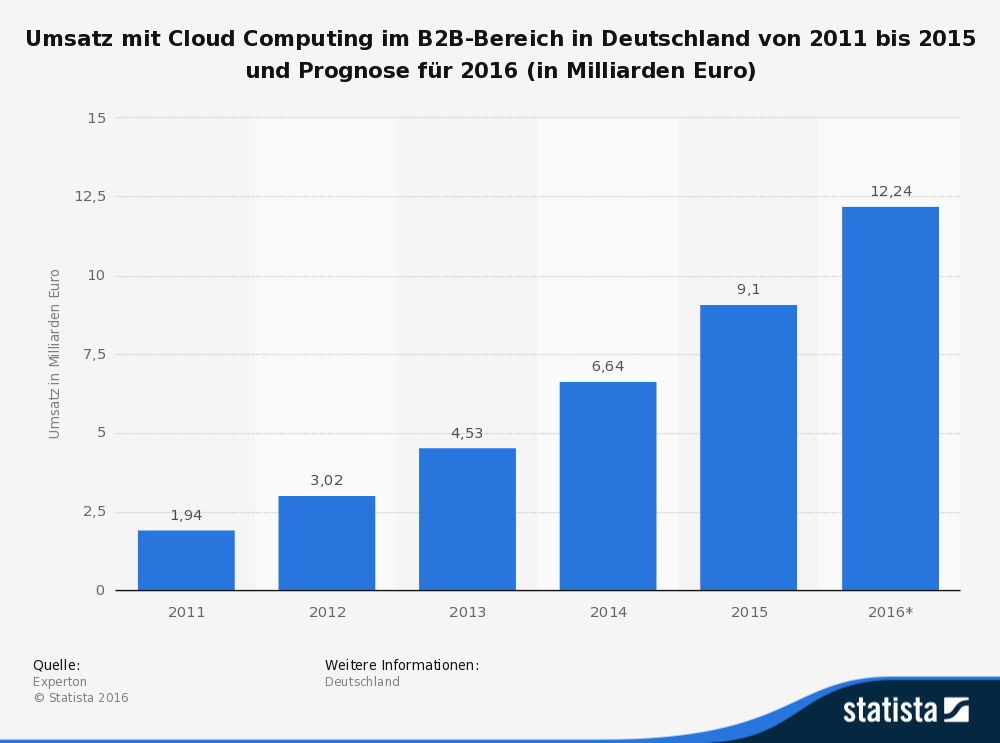
\includegraphics[scale=0.5]{images/cloud-computing-market}
	\caption{Umsatz mit Cloud Computing im B2B-Bereich in Deutschland von 2011 bis 2015 und Prognose für 2016 \parencite{statistia.2015}}
	\label{fig:cloudmarket}
\end{figure}

Wie man \autoref{fig:cloudmarket} entnehmen kann, passen sich die verschiedenen Vendoren an die neuen Herausforderungen an und fokussieren immer mehr auf den Cloud-Computing-Markt.

Leider entstehen hierdurch wieder neue Probleme: Die Kontrolle über nutzerspezifische Daten geht verloren. Durch das Deployment der Anwendung auf verschiedene Server und die Verteilung der Daten auf verschiedene Datenbanken ist es für den Nutzer schwierig geworden, den Datenweg nachzuvollziehen.

Dies wird besonders zum Problem, wenn rechtlich geschützte Daten in der Cloud verwendet werden sollen. Ebenfalls gibt es sensitive Geschäftsdaten, die Firmen nur ungern aus der Hand geben möchten und die nicht ins unsichere Internet gelangen dürfen.
Zum Teil kann dies durch bessere Sicherheitslösungen und Verschlüsselung behoben werden, aber oft müssen zumindest die Datenbanken beim Kunden vor Ort bleiben. 

Um auch diesen Anforderungen gerecht zu werden, entstehen immer häufiger so genannte Hybrid Cloud Modelle. Bei diesen findet ein Teil der Geschäftsprozesse in der öffentlichen Cloud statt und sicherheitskritische Softwareteile werden lokal vom Nutzer selbst gehostet. Ebenfalls besteht bei diesen Lösungen die Möglichkeit, dass Performance Spitzen in der Cloud bearbeitet werden, sodass spontan zusätzliche Leistung alloziert werden kann.

Im Kontext dieser Arbeit soll untersucht werden, inwiefern eine Cluster Speicherlösungen an eine Public Cloud angebunden werden kann, sodass Daten direkt mit der Cloud geteilt und dort analysiert werden können. 

\section{Aufgabenstellung}\label{sec:tasks}
\subsection{Umfeld} \label{subsec:enviroment}

\begin{wrapfigure}{r}{0.35\textwidth}
	\begin{center}
		
\includegraphics[width=0.32\textwidth]{images/firma-deckblatt}
	\end{center}
	\caption{Firmenlogo des Ausbildungsbetriebs IBM Deutschland GmbH}
\end{wrapfigure}

Diese Bachelor-Arbeit begleitet ein zwölfwöchiges Praktikum bei der Ausbildungsfirma IBM Deutschland GmbH. Bestandteile der Thesis sind die praktischen Implementierungen und die zugehörige Recherche innerhalb des Betriebs. 

Bei IBM wird die Arbeit in dem Bereich EMEA Storage Competence Center (ESCC), speziell in der Abteilung Infrastructure \& Lab Solutions, angefertigt. Diese ist im IBM-Standort Kelsterbach in Hessen angesiedelt, an welches auch ein Speicherlabor angeschlossen ist.

Aufgabe der Abteilung ist das Management und die Erstellung von Labordemonstrationen mithilfe von verschiedenen Server-, Speicher- und Softwarelösungen. Diese werden dann verwendet, um Funktionalitäten von IBM-Speicherprodukten etwaigen Kunden vorzuführen.

\subsection{Ist-Zustand}

In der Abteilung werden zur Zeit verschiedene lokale Speicherlösungen von IBM in Testumgebungen zur Verfügung gestellt. Auch komplexe Lösungen, wie zum Beispiel Spectrum Scale, können in virtuellen Speicherclustern realistisch simuliert werden. Besonders neue Features sollen hierbei vorgeführt werden.

Aufgrund vieler relativ alter Produkte, die schon seit Jahrzehnten stets weiterentwickelt wurden, gibt es nur wenige mit öffentlichen Cloud-Dienstleistern zusammenspielende Demoanwendungen.

Ebenfalls werden vereinzelt ältere Versionen von Software verwendet, die noch keine oder nur teilweise Anbindung an Cloud-Dienste ermöglichen. 

Die Anzahl an Demoanwendungen, die direkt in der Cloud laufen und auf die lokalen Lösungen zugreifen, ist leider ebenfalls noch relativ gering. 

\subsection{Soll-Zustand}

Langfristig ist die Bereitstellung viele Demos für Cloud-Szenarien ein wichtiges Ziel der Abteilung. Diese sollen auf der einen Seite die Kompatibilität von IBM-Produkten mit verschiedenen Cloudanbietern verdeutlichen und auf der anderen Seite Synergien mit kognitiven Diensten von IBM aufzeigen.

Das Potential vieler Produkte, private, hybride und öffentliche Cloud Computing Lösungen zu ermöglichen, soll nicht nur in der Theorie vorhanden sein, sondern hier aktiv präsentiert und implementiert sein.

Dies ist nur möglich, wenn eine größere Anzahl an Demos zur Verfügung gestellt wird, die im besten Fall auf \gls{Bluemix} laufen, damit auch die Fähigkeiten vom IBM Cloud Angebot gezeigt werden können. 

\subsection{Aufgaben}

Im Rahmen dieser Arbeit soll das Clusterspeichersystem Spectrum Scale (früher GPFS) mit einer Public Cloud-Lösung verknüpft werden. Hierzu sollen die vorhandenen Möglichkeiten der Software für diesen Anwendungsfall untersucht und evaluiert werden.
Die Geeignetste soll innerhalb einer Testumgebung aufgesetzt, konfiguriert und mit einem geeigneten Speicher in der Cloud erweitert werden. 
Sollte sich das Setup als sinnvoll erweisen, besteht die Möglichkeit, diese Umgebung in einer Produktivumgebung im Labor einzurichten.

Zusätzlich soll eine Demonanwendung entwickelt werden, die das Potential des oben beschriebenen Setups testen kann. Diese Anwendung sollte ebenfalls in \gls{Bluemix} entwickelt werden, sodass eine echte Hybrid Cloud-Applikation entsteht. 

Diese soll eine Technik (Cloud Sharing) darstellen, mithilfe der Daten aus einem lokalen System in Cloud betrachtet und bearbeitet werden können.

Die Einbindung von weiteren IBM-Diensten ist hierbei erwünscht, damit mögliche Anwendungen für Kunden besser dargestellt werden können.

\subsection{Rahmenbedingungen und Abgrenzung}

Sämtliche Arbeit findet innerhalb der in \autoref{subsec:enviroment} erwähnten Abteilung statt. Hierbei wird ebenfalls Fachwissen von den Mitarbeitern zur Unterstützung und Beratung hinzugezogen.

Software und Hardware zum Aufsetzen von IBM Produkten wird bereitgestellt, hierbei speziell IBM Spectrum Scale. Für die Entwicklung mithilfe einer Testumgebung wird ein Lenovo Thinkpad T440 mit Redhat 7.3 Linux verwendet. Hierbei wird der Clusterspeicher in einer mit KVM betriebenen virtuellen Maschine aufgesetzt.

Zur Versionsverwaltung der Demoanwendung wird \gls{Git} verwendet. Notwendiges Projektmanagement wird agil umgesetzt und es werden, wenn notwendig, Stories oder auch Tasks erzeugt, die dann zusammen mit den Git Issues getrackt werden können (ein Feature von der Gitumgebung von Bluemix).

Zudem werden eine Reihe externer Tools und Frameworks eingesetzt, ebenso wie IBM Software, die verwendet und angepasst wird und nicht direkter Teil dieser Arbeit ist. Ich beschränke den Bericht auf von mir gemachte Entwicklung, außer diese steht im direkten Zusammenhang mit Features, die von Anderen implementiert wurden und aus Verständlichkeitsgründen nicht ausgelassen werden können.

IBM Spectrum Scale wird nicht komplett aufgesetzt, da dies zeitaufwendig und bereits häufig gemacht worden ist. Stattdessen wird ein konfiguriertes Abbild verwendet, dass nur noch für die Verwendung mit der Cloud verändert werden muss.

Ich erhebe keinen Anspruch auf die Arbeit Anderer, auch wenn an manchen Stellen die Vorarbeit von Kollegen aus der Abteilung verwendet wird. Entsprechende Stellen werden eindeutig gekennzeichnet und angemessen begründet.

\section{Struktur der Arbeit}
Der Aufbau der Arbeit sollte anhand der Gliederung leicht erkennbar sein, wird hier aber noch einmal im Detail dargestellt. Im \autoref{ch:introduction} wird die Motivation der Arbeit, ihr Kontext und die spezifische Aufgabenstellung dargelegt.

Im \autoref{ch:background} werden verschiedene heutzutage relevante Technologie für Speicher, verteilte Speichersysteme und Cloud Computing diskutiert. Sie bilden die Grundlage für die Auswahl der relevanten Tools, speziell im Cloud-Umfeld, für die Umsetzung der Aufgaben unter Berücksichtigung der besonderen Vorzüge des Ausbildungsunternehmens.
An dieser Stelle werden auch sämtliche relevanten Begriffe, Konzepte und Lösungen gezeigt, die notwendig sind, um sich in das behandelte Themenumfeld einzuarbeiten.

Eingehend auf oben erwähnte Beschränkung wird dann im \autoref{ch:methods} eine Auswahl an Umgebungen und Werkzeugen getroffen und verwendete Techniken zum Entwickeln beschrieben.

Resultate und der Ablauf der Entwicklung werden im \autoref{ch:realization} beschrieben. Dabei werden sowohl überwundene Probleme, wie auch die Gesamtarchitektur der Lösung dargelegt.

Zum Abschluss der Arbeit (\autoref{ch:conclusion}) werden diese Ergebnisse kritisch diskutiert und es wird ein Ausblick auf mögliche zukünftige Entwicklungen im Bereich des Hybrid Cloud Computing gegeben.
	
	% Theoretische Grundlagen
	\chapter{Stand der Technik}\label{ch:background}

Zum Aufsetzen einer Hybrid Cloud-Umgebung und dem Entwickeln einer auf dieser laufenden Anwendungen werden verschiedene Grundlagen benötigt. Grundwissen über die unterschiedlichen Speichertypen ist notwendig, um die Herausforderungen eines verteilten Speichersystems zu verstehen. Ebenfalls ist fundiertes Wissen über die Cloud, ihre Umsetzung und Typen wichtig, um in der Lage sein, effiziente Anwendungen für diese zu entwickeln.

In diesem Kapitel werden diese Hintergründe erläutert.

\section{Speicherlösungen} \label{sec:storage}
Speicherung von Daten ist ein wichtiges Thema in der IT, wodurch unzählige Technologien entstanden sind. Hier werden erst Hardwarespeicher beschrieben und danach verschiedene Arten, diesen innerhalb von Rechnernetzwerken zusammenzustellen.

\begin{figure}[hbt]
	\centering
	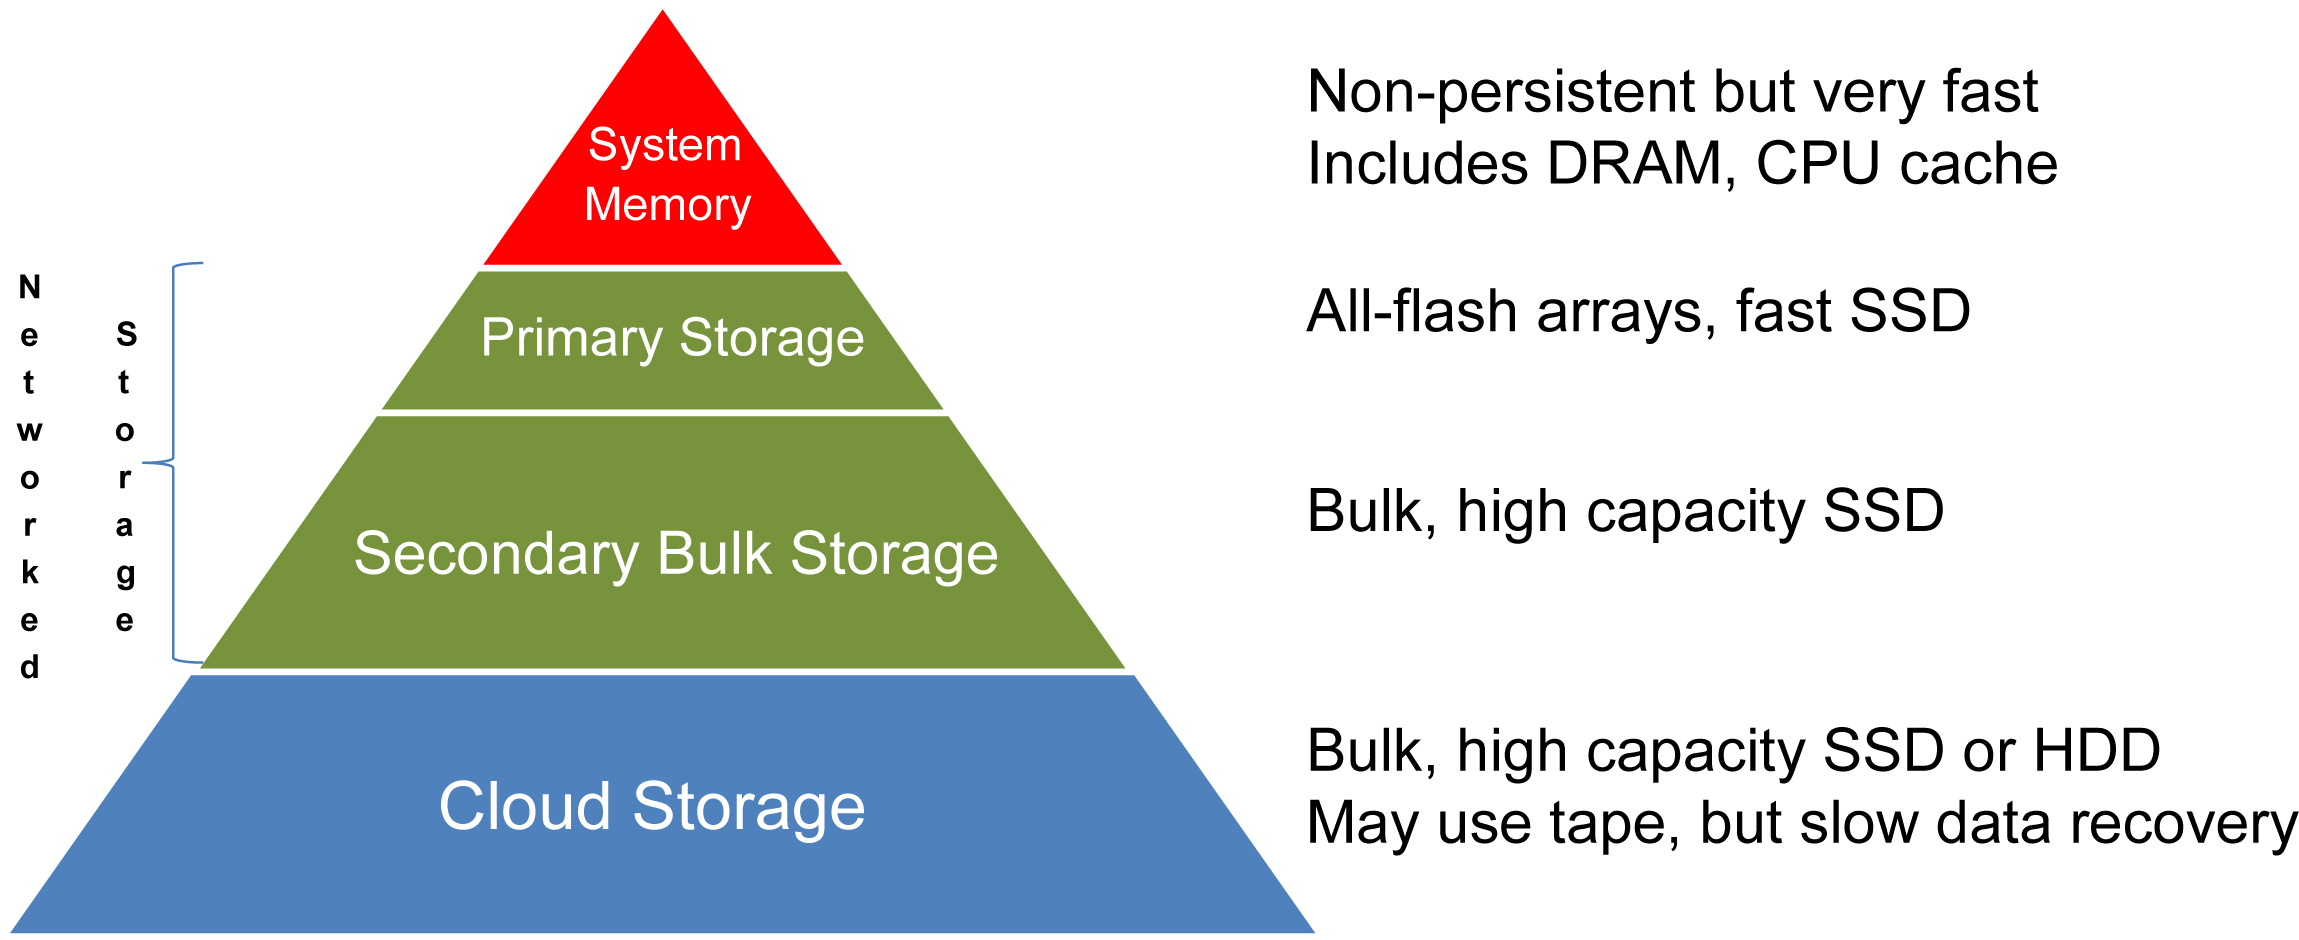
\includegraphics[scale=0.75]{images/storage-pyramide}
	\caption{Speicherpyramide \parencite{kaufmann.2016}}
	\label{fig:storagepyramide}
\end{figure}

Prinzipiell kann Speicher immer in eine Art Hierarchie eingeteilt werden. Extrem häufig verwendete Daten landen auf der ersten Ebene. Diese wird meistens in Form von Cache oder RAM bereitgestellt und bietet extrem kurze Latenz, aber nur geringen Speicherumfang.

Auf der nächsten Ebene stehen schnelle Speichermedien, zum Beispiel SSDs. Direkt darunter ordnen sich klassische Festplattenspeicher ein, die den Großteil des Speichervolumens zur Verfügung stellen. Sie haben höhere Latenzen, sind aber dafür günstig und haben eine hohe Kapazität \parencite[Kap. 2, What is Computer Storage?]{kaufmann.2016}.

Mit der letzten Stufe ``Cloud Speicher'' wird sich intensiver in der \autoref{sec:cloud} auseinander gesetzt.

\subsection{Hardware}

Unabhängig von der Zusammenstellung umfänglicher Speicherlösungen, müssen die Daten trotzdem irgendwann auf einen Hardwarespeicher geschrieben werden. Folgender Abschnitt erläutert, die allgemeine Funktion und geht auf einige der häufigsten verwendeten Typen ein.

\subsubsection{Hard Disk Drive (HDD)}

Hierbei handelt es sich um einen nicht volatilen Speicher, der digital kodierten Inhalte auf der magnetischen Oberfläche einer Platte speichert. Traditionell gibt es zwei Protokolle: SAS im kommerziellen und SATA im privaten Sektor \parencite{wikibooks.2016}.

Ein oder mehrere Leseköpfe werden mithilfe von Armen und einem Servomotor über die Platte bewegt, um relevante Stellen auszulesen. Bei der Herstellung von HDDs werden Tracks in die Platte geschrieben, die jeweils ein Label und Blockinformationen besitzen. Durch sie ist es einfacher, den Lesekopf zu platzieren. Jeder dieser Tracks kann bis zu einigen MBs an Daten beinhalten. Durch die Blockbildung bei I/O-Operationen kann häufig nur ein einzelner Block (64-256) geschrieben werden, wodurch Festplatten unnötig langsam werden. Durch neue Technologie können IOs in eine Warteschlange eingereiht werden, sodass die Platte kontinuierlich lesen und schreiben kann. Trotzdem ist nur eine maximale Geschwindigkeit von ungefähr 300 \gls{IOPS} das Limit für Platten mit 10.000 RPM \parencite[Kap. 3]{kaufmann.2016}.

Jede Festplatte hat heutzutage einige private Sektoren, auf denen Reparaturinformationen und Reserveblöcke gespeichert sind. Fällt ein Block in der Festplatte aus (durch zum Beispiel physikalische Beschädigung), kann dieser fließend ersetzt werden, sodass keine Daten verloren gehen. Kurz vor dem Ausfall einer Platte steigt diese Anzahl der Lesefehler einer Platte massiv an, sodass eine Datenreovery versucht werden kann. Leider ist dies keine verlässliche Methode, um Daten zu sichern, sodass andere Methoden verwendet werden sollten \parencite[Kap. 3]{kaufmann.2016}.

Um Datenverlust durch Plattenausfälle entgegenzuwirken, besteht die Möglichkeit der Verwendung von so genannten RAIDs. Dies ist eine Methode, bei der mehrere HDDs so zusammengeschaltet werden, sodass bei dem Ausfall einer Einzelnen die Daten weiterhin verfügbar sind \parencite{wikibooks.2016}.

Festplatten sind gut erforscht, es treten extrem selten unbekannte Probleme auf und werden seit Jahrzehnten verwendet, ihr Speicher ist extrem günstig geworden und in Masse verfügbar. Ihr größter Nachteil ist eine sehr geringe I/O-Geschwindigkeit im Vergleich mit neueren Technologien \parencite[Kap. 3]{kaufmann.2016}.

\subsubsection{Solid State Drive (SSD)}

Im Jahr 2007 wurde der erste SSD-Speicher vermarktet und stach durch extrem hohe Zugriffszahlen heraus. Diese waren bei 4000 \gls{IOPS} bereits um das zehnfache höher als die klassischer Festplatten. Heutzutage ist es möglich IOPS Zahlen im Millionenbereich zu erreichen, was eine Revolution für Speicher bedeutet \parencite[Kap. 3]{kaufmann.2016}.

\begin{figure}[hbt]
	\centering
	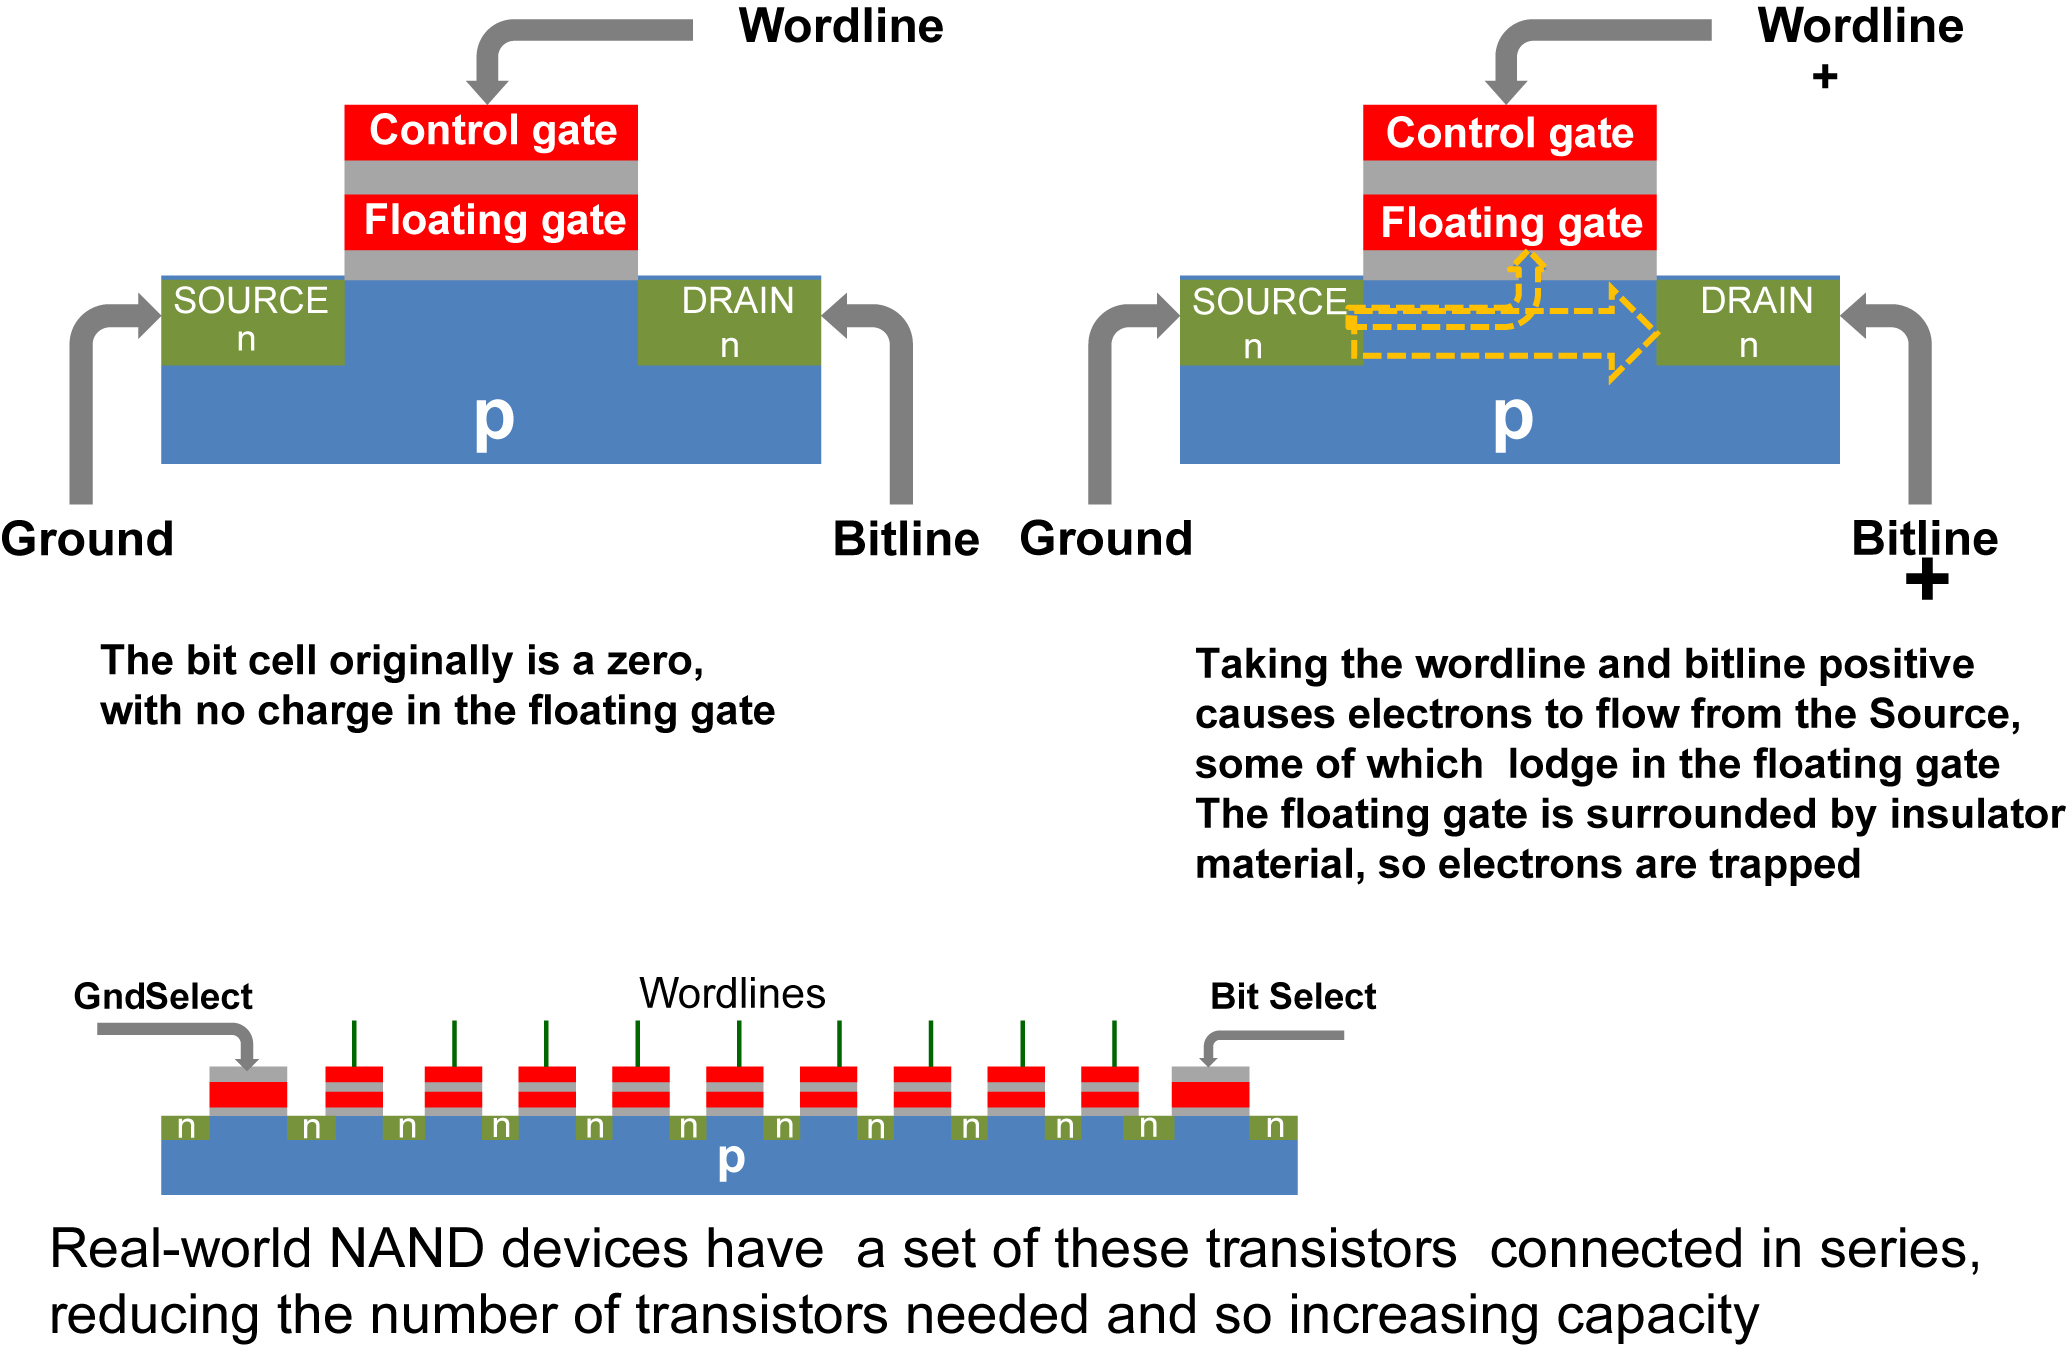
\includegraphics[scale=0.85]{images/flash}
	\caption{Funktionsweise eines NAND-Flashspeichers \parencite{kaufmann.2016}}
	\label{fig:flash}
\end{figure}

SSDs benutzen Nicht-Und (NAND) memory chips zum Speichern einzelner Bitinformationen. Von diesen Zellen gibt es dann einige Millionen, die beliebig adressiert werden können (Random Access Memory). Innerhalb eines so genannten Floating Gate können nun Elektronen eingefangen werden, um eine binäre Eins zu repräsentieren. Im Ausgangszustand sind diese ``Fallen'' leer, um einen Nullinformationen zu speichern. Sobald der Speichercontroller eine Zelle laden will, wird der Einlasstransistor geöffnet und einige Elektronen in der Zelle für eine beliebig lange Zeit gefangen.

Dieser Prozess findet in \autoref{fig:flash} statt, wenn auf der Bit- und Wordline eine positive Ladung gesetzt wird. Meistens liegen mehrere Zellen auf einer Reihe, was den Leseprozess verkomplizieren kann. Es wird eine niedrige Spannung an alle Wordlines angelegt, wodurch bei geladenen Zellen eine Konduktivität festgestellt werden kann. 

Wird eine einzelne Zelle zu häufig beschrieben, kann diese Isolation verlieren, wodurch sie unnutzbar zum Speichern wird. Schreibstrategien und Reservezellen werden verwendet, um dem vorzubeugen.	

Zum Löschen der Zellen wird eine hohe negative Spannung an die Zellen angelegt, wodurch die gefangenen Elektronen aus den Floating Gates heraus gestoßen werden. Dies passiert meistens in fest definierten Pages, sodass keine speziellen Blöcke gelöscht werden können. Nach dem Löschen eines Blockes wird dessen Zeiger auf eine vorher geleerte Page bewegt und der Block als ``discared'' markiert. Sind innerhalb einer Page genug Blöcke in diesem Zustand, werden die verbleibenden Daten verschoben und die gesamte Page gelöscht und Teil des freien Speichers der SSD \parencite{kaufmann.2016}. 
Durch diesen Prozess ist das Löschen von Dateien nicht mehr zuverlässig, da die Daten noch für lange Zeit innerhalb eines ``discared'' Blockes liegen können, der erst wesentlich später vom Controller gelöscht wird.

SSDs können über das SATA-Protokoll angeschlossen werden, aber in den letzten Jahren wurde das wesentlich performantere NVMe entwickelt.

Da dieser Speicher keine sich bewegenden Teile hat, ist er wesentlich robuster was Schläge, Vibrationen und hohe Temperaturen angeht. Ebenfalls ist der Strombedarf wesentlich geringer, was zusammen mit den vorherigen Punkten den Betrieb von SSDs in großen Rechenzentren wesentlich einfacher und günstiger macht.

Trotzdem gibt es auch einige Nachteile von Flashspeicheren: Die meisten Anwendungen sind nicht darauf ausgelegt, so hohe Zugriffszahlen zu unterstützen. In der Vergangenheit hat I/O immer ein Bottleneck in Applikationen dargestellt, sodass die meisten Programme entsprechend designed wurden.
Dies zieht sich durch die gesamte Softwarelandschaft und auch die geläufigen Betriebssysteme sind nicht in der Lage, diese neue Geschwindigkeit voll auszunutzen. Ebenfalls ist das SATA Interface nicht perfekt für SSDs, da es ursprünglich dafür designed war, die niedrigen Bandbreiten von Festplatten auszugleichen \parencite[Kap. 3]{kaufmann.2016}.


\subsubsection{Bandlaufwerk}

Bandlaufwerke funktionieren im Grunde wie die früher verwendeten Kassetten. Innerhalb des Laufwerkes befindet sich ein dünner Streifen aus Plastik mit einer magnetischen Oberfläche. Dieser wird, ähnlich wie bei Festplatten, mit digitalen Daten beschrieben. 

Es kann nicht auf beliebige Bereiche des Bandes zugegriffen werden, Lesen und Schreiben erfolgt immer sequentiell. Das Laufwerk muss von Anfang bis Ende durchlaufen werden, um I/O Aktionen durchführen zu können \parencite{adrc.2009}.

Ein Bandlaufwerk verwendet einen kleinen Motor, um das Band auf- und abzuwickeln. Dabei wandert dieses entlang eines Lese- und Schreibkopfes. Um Unterschiede zwischen der Geschwindigkeit der ankommenden Daten vom Computer und der begrenzten \gls{IOPS} des Laufwerkes auszugleichen, wird eine Steuereinheit verwendet. Diese regelt Fehlerhandling, Puffer und andere logische Operationen.

Informationen werden in die Steuereinheit geladen und dann auf das Band geschrieben. Dieser Prozess wiederholt sich solange, bis keine Daten mehr vorhanden sind.

Aufgrund von geringen Kosten und hoher Lebenszeit wird diese Art von Laufwerk immer noch häufig verwendet. Besonders of wird es für Backupszenarien genutzt, da hier die Nachteile des nur sequentiellen Zugriffes auf Daten keine große Rolle spielen \parencite{adrc.2009}. 

\subsection{Speicheranbindung über Netzwerke}
\subsubsection{Direct Attached Storage (DAS)}

Bei \ac{DAS} handelt es sich um externen Speicher, der direkt mit einem oder mehreren Servern über ein \gls{SCSI} Interface verbunden ist. Dabei wird kein Netzwerk verwendet. Es gibt verschiedene Typen von \ac{DAS}, bei manchen werden nur beliebige Platten zusammengewürfelt (\ac{JBOD}), bei anderen ganze Plattenarrays angeschlossen.
Hierbei handelt sich um den ältesten Speichertypen, der lange vor dem Entstehen von SAN oder NAS verwendet wurde.

Es kann nur eine begrenzte Anzahl von \ac{DAS} an einen Rechner angeschlossen werden, da die Anzahl von SCSI-Schnittstellen an Servern limitiert ist. Dadurch ist diese Art von Speicher leider nur begrenzt skalierbar.

Ein weiterer großer Nachteil von direkt angebundenen Speicher ist, dass bei einem Ausfall des Servers ein wesentlicher Teil der Daten nicht mehr erreichbar ist. Die Verfügbarkeit der Daten hängt also nicht nur vom Speicher selber ab, sondern auch von dem bereitstellenden Server.

Wird das Laufwerk an mehrere Server angeschlossen, um obige, Problem entgegenzuwirken, erhöht sich durch einen Ausfall die Zugriffszeit beträchtlich \parencite[Kap. 1, Disk Storage Systems]{gupta.2002}.

Der größte Vorteil von DAS Geräten ist, dass sie einfach aufzusetzen und zu warten sind, da keine Netzwerkkenntnisse oder Hardware benötigt werden. Dies bedeutet geringe Kosten und einfache Handhabung \parencite{beal.2017}.

\subsubsection{Network Attached Storage (NAS)}

\ac{NAS} ist ein einfaches System, um Daten an einer einheitlichen Stelle im Netzwerk zu speichern. Hierdurch werden die Daten von den Servern selber zu speziell zur Speicherung ausgelegten Hardware wegbewegt. 

Ein NAS-Gerät ist spezialisierte Hardware mit meist zugehöriger Management Software. In den meisten Fällen muss es nur mit dem Firmennetzwerk verbunden und eingeschaltet werden. Ebenfalls ist der Speicher plattformunabhängig und kann mithilfe verschiedener Protokolle von jedem Client verwendet werden. Einige Beispiele für diese sind: HTTP (Internetanfragen), FTP oder TCP/IP. Ebenfalls können Datenanfragen über NFS (für Linux) oder SMB (für Windows) getätigt werden \parencite[Kap. 1, NAS Devices]{gupta.2002}.

Bei einem Daten Request wird die Anfrage an das NAS Gerät weitergeleitet, das die notwendige Daten an den Server zurück sendet, welcher diese dem Client zur Verfügung stellt.

NAS besitzt einige Vorteile: Es gibt eine deutliche Leistungssteigerung bei den Anwendungsservern, da I/O Operationen komplett auf der dedizierten Hardware ausgeführt werden. NAS Devices besitzen eine wesentlich bessere Skalierbarkeit als \ac{DAS} Geräte, es können beliebig viele neue Netzwerkspeicher zu einem System hinzugefügt werden.

Ebenfalls ist die Fehleranfälligkeit wesentlich geringer, wenn ein Anwendungsserver abstürzt, bleibt der Zugriff auf den NAS im Netzwerk immer noch erhalten.

Management und Einsatz sind auch einfach gehalten, die Geräte konfigurieren sich zu großen Teilen selber und sind mit jedem System ansprechbar.

Trotz all dieser Vorteile gibt es, besonders in großen Netzwerken, auch einige Nachteile. Anfragen von Clients erzeugen eine große Menge Netzwerkverkehr, der viel Bandbreite beansprucht. Sobald viele Request gleichzeitig auftreten, kann es deswegen auch zu Performanceeinbrüchen kommen.

Durch die Zentralisierung des Speichers wird dieser auch einfacher anfälliger für bösartige Attacken, Netzwerk Verkehr kann abgefangen oder modifiziert werden \parencite[Kap. 1, Adv. and Disadv. of NAS Devices]{gupta.2002}.


\subsubsection{Storage Area Network (SAN)}
\ac{SAN} wurden entwickelt, um enorme Mengen an Daten zu verarbeiten. Sie werden nicht direkt in das Client- oder Servernetzwerk eingebunden, sondern bilden ein eigenes, das die verschiedenen Speicher miteinander verbindet. Dieses kann dann nur durch die SAN Server angesprochen werden. Dies führt zu einem sehr sicheren Setup, da die Geräte vor den Clients komplett verborgen sind \parencite[Kap. 1, SANs]{gupta.2002}.

Es gibt mehrere wichtige Bestandteile: Die oben erwähnten Server stellen den Zugriffspunkt für Applikationsserver im normalen Netzwerk. Innerhalb des Netzwerks kann es verschiedene Speichertypen geben (RAIDs, JOBDs, Disk Storage Systems, Bandlaufwerke).
Interfaces werden verwendet, um den Speicher mit den Server zu verbinden und sie damit zu externalisieren. Mithilfe von SAN Interconnects können entfernte Speicher ebenfalls eingebunden werden. Hubs und Router werden benutzt, um verschiedene Speicher zusammenzuschließen, wobei Router das Signal immer nur zu einem Gerät weiterleiten und es nicht broadcasten.
Außerdem gibt es noch eine ganze Reihe an weiteren Geräten, die für die Kommunikation zwischen verschiedenen Protokollen und Technologien verantwortlich sind \parencite[Kap. 2, SAN Components and Building Blocks]{gupta.2002}.

Ein vereinfachtes Setup kann in \autoref{fig:storageareanetwork} betrachtet werden.

\begin{figure}[hbt]
	\centering
	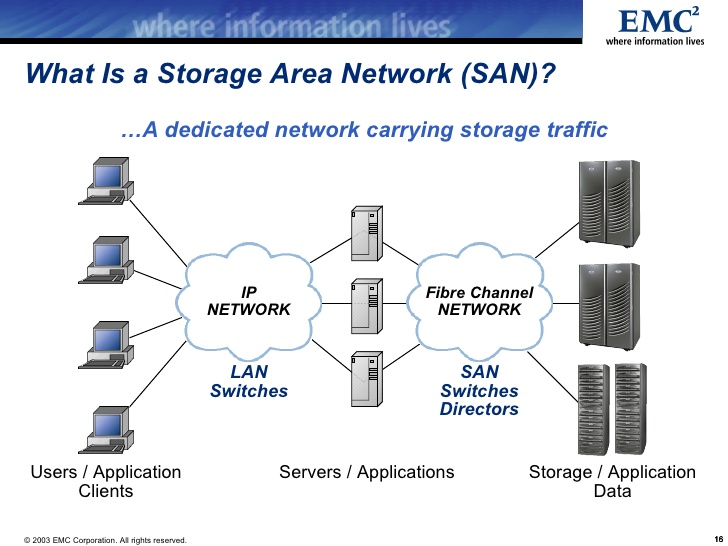
\includegraphics[scale=0.9]{images/storage-area-network}
	\caption{Typische SAN Konstruktion \parencite[Kap. 1]{gupta.2002}}
	\label{fig:storageareanetwork}
\end{figure}

Durch dieses eigene Netzwerke können einige Vorteile ausgenutzt werden, die so bei \ac{NAS} nicht oder nur schwer zu erreichen sind. Zur Verbindung der Geräte können Hochleistungsnetzwerke wie FibreChannel verwendet werden, die wesentlich performanter sind als Ethernet. Da das SAN getrennt vom Netzwerk der Applikationsserver ist, muss keine Bandbreite geteilt werden, was ebenfalls die Anwendungen schneller macht. Genauso wie bei NAS werden I/O-Aktionen auf die SAN-Geräte verlagert und es können zusätzlich Performance intensive Backups isoliert im SAN erledigt werden \parencite[Kap. 1, SANs]{gupta.2002}.

Das Filesystem von SANs wird nicht von den Geräten selber verwaltet, sondern von den entsprechenden Fileservern. SANs bieten einfachen Blockzugriff auf die Daten, für die Server sind sie nur weitere Festplatten. Dadurch ist es einfacher, das SAN beliebig zu skalieren, da einfach nur neue Speichergeräte hinzugefügt werden müssen. Die Ausfallsicherheit wird ebenfalls höher, da meistens verschiedene Server Zugriff auf das SAN haben und einfach ein weiterer angesprochen werden kann, falls ein Ausfall stattfindet.

Es gibt optimierte Software zur Verwaltung von SANs, die höhere Performance ermöglichen.

Ein großer Nachteil von SANs ist, dass sie sehr komplex aufzusetzen sind und auch die Kosten wesentlich höher sind als bei NAS Lösungen \parencite[Kap. 2]{gupta.2002}.

\newpage

\section{Verteilte Dateisysteme} \label{sec:filesystems}

Für Anwendungen und Nutzer organisiert ein Dateisystem eine abstrahierte Sicht auf sämtlichen Daten. Es stellt eine Schnittstelle für Online-, Offline- und Programmzugriff zur Verfügung. Ein Filesystem besteht aus einer Sammlung aller Dateien und einer Ordnerstruktur, die erstere organisiert und beschreibt. 

Das Betriebssystem ordnet Speicherblöcke logischen Einheiten zu, so genannten \textbf{Files}. Die physikalischen Eigenschaften des Speichergerätes werden hiermit vor dem Nutzer verborgen. SSDs, HDDs, Onlinespeicher und sogar Cluster-Dateisysteme können hierdurch auf die gleiche Art betrachtet werden \parencite{silberschatz.2012}.

Im Folgenden werden verschiedene Clusterdateisysteme mit ihre Vor- und Nachteile untersucht. Dabei wird besonderer Wert auf die Kompatibilität mit Cloud Lösungen gelegt. Ebenfalls liegt ein stärker Fokus auf der Lösung von IBM, die Gründe hierfür werden im \autoref{ch:methods} näher erläutert.

\subsection{IBM Spectrum Scale - GPFS}

Bei IBM Spectrum Scale handelt es sich um ein System, dass den gleichzeitigen Zugriff auf ein oder mehrere Dateisysteme zur Verfügung stellt von verschiedenen Knoten. Diesen können mithilfe von unterschiedlichsten Techniken den Zugriff zur Verfügung stellen (SAN, NAS, DAS) und ermöglichen das Aufsetzen von einem hochperformanten skalierbaren Netzwerkes \parencite[S. 1]{ibm.2017}.

Neben einfachen Datenzugriff werden ein Vielzahl von zusätzlichen Features geboten: Datei Duplizierung, Regel basiertes Speicher Management, Kommunikation und Zusammenschluss verschiedener Rechenzentren und diverse andere. Auf diese wird hier aber nur sehr grob eingegangen, da sie größtenteils unrelevant für die Arbeit sind und deren Umfang übersteigen würden.

\textbf{Hauptkomponenten und Funktionen}

Von jedem Knoten des Clusters kann gleichzeitig auf sämtliche Daten zugegriffen werden. Aufgrund der \gls{POSIX} Kompatibilität kann der Zugriff über Systemfunktionen (open, read, write) oder speziellen APIs erfolgen. Dies vereinfacht die Bedienung erheblich, da der Cluster für den einzelnen Rechner wie eine ``normale'' Festplatte erscheint. Auf jedem GPFS Knoten sind drei Hauptkomponenten installiert:

\begin{itemize}
	\item \textbf{GPFS Administration Kommandos} \\
	Eine Reihe von Skripts und Programme, die Konfigurationen ändern und Operationen auslösen können. Ausgeführte Kommandos können beliebige Knoten betreffen und werden entsprechend weitergeleitet und auf entfernten Systemen ausgeführt.
	\item \textbf{GPFS Kernel Erweiterung} \\
	Diese Erweiterung bietet ein Interface zum Betriebssystem und ermöglicht es GPFS als natives Dateisystem zu registrieren. Hierdurch erscheint der gesamte Cluster für eine Applikation wie eine einzelne Festplatte. Der Kernel führte diese entweder lokal auf verfügbarem Speicher aus oder leitet sie mithilfe des GPFS Daemon zu anderen Geräten weiter.
	\item \textbf{GPFS Daemon} \\
	Aufgabe dieses multithreaded Programmes ist das Ausführen sämtlicher Schreib-, Lese- und Pufferaktionen. Er sorgt auch für die Datenkonsistenz des Gesamtsystems. Zusätzlich zu den I/O Aktionen wird auch die Kommunikation mit anderen Knoten im System ausgeführt, um Konfigurationsänderungen, Wiederherstellung und parallele Updates durchzuführen.
	Ebenfalls enthalten ist die Network Shared Disk Komponente, die Cluster weite Benennung von und den Zugriff auf Speicher zur Verfügung stellt \parencite[S. 6]{ibm.2017}.  
\end{itemize} 

\textbf{Cluster Arten}

Es kann eine Vielzahl von Cluster Konfigurationen erreicht werden, da Spectrum Scale unterschiedlichste Betriebssysteme unterstützt (speziell Linux, AIX, Windows) und Speicher auf verschiedene Arten anschließbar ist. Im Folgenden werden zwei häufige Szenarien vorgestellt.

Eine Variante ist der Anschluss von sämtlichen Knoten an das selbe Storage Area Network. Ist dies nicht der Fall, können nur einzelne Nodes angeschlossen sein als \ac{NSD} Server und die verbleibenden sind \ac{NSD} Klienten. Hierbei wird eine klassische Server-Client Architektur aufsetzen bei der eine Vielzahl von GPFS Klienten auf eine kleinere Anzahl von GPFS Servern mit Speicheranbindung zugreift \parencite[S. 8]{ibm.2017}.

\begin{figure}[hbt]
	\centering
	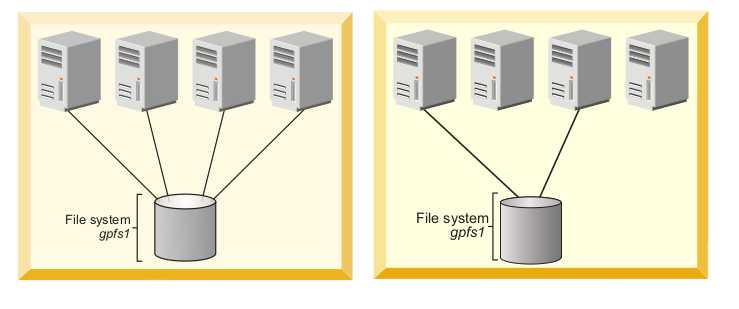
\includegraphics[scale=0.6]{images/gpfs-architectures}
	\caption{Anbindung an alle Knoten (links) und Server-Klient Architektur (rechts) \parencite[S. 8]{ibm.2017}}
	\label{fig:gpfsarchitecture}
\end{figure}

\textbf{Verbindung mit Cloud Diensten}

Cloud Dienste mit Spectrum Scale bieten zwei Funktionsweisen: \textbf{Cloud Tiering} und \textbf{Data Sharing}. Es können maximal vier verschiedene Knoten und ein Dateisystem für diese Dienste verwendet werden \parencite{mani.2017}.

Im ersten Szenario werden so genannte kalte Daten (also Dateien, die selten benutzt werden und geringe Zugriffszahlen haben) in der Cloud gespeichert, um die schnellen lokalen Datenspeicher zu entlasten. Dadurch kann die Clusterperformance erhöht und kosten für zusätzlichen Speicher gespart werden. Diese Funktion ist das Information Lifecycle Management (\ac{ILM}) System eingebunden und ermöglicht es den Administratoren Strategien zu definieren, um die Auslagerung bei bestimmten Daten auszulösen.
Es sollten nur kalte Files in der Cloud gespeichert werden, da diese bei Zugriff zu downloaden sind, was die Latenz massiv erhöht \parencite[S. 107]{ibm.2017}.
Lokal wird ein Cloud Verzeichnis angelegt, welches alle migrierten Daten auflistet. Wird auf einen Datei-Stub zugegriffen, kann die ferne Information heruntergeladen werden. In der Cloud liegen pro File zwei verschlüsselte Dateien, eins für die eigentlichen Daten und ein zweites mit Metadaten (Besitzer, Zugriff, ...) \parencite[S. 108]{ibm.2017}.

Beim Cloud Sharing ermöglicht das Teilen von lokalen Daten mit verschiedenen Arten von Objekt Speichern (\autoref{subsec:objectstorage}). Dieser Export kann ebenfalls durch IML Strategien in regelmäßigen Zyklen ausgelöst werden, um zum Beispiel Daten in der Cloud aktuell zu halten. Diese können dann von anderen Applikationen verwendet werden. Es ist ebenfalls ein Import von Object Storage System möglich, um die lokalen Daten ggf. zu erweitern.
Der Export wird parallel mit allen Cloud Dienst Knoten durchgeführt. Dabei kann eine Liste aller Daten in einem Manifest gespeichert werden, um diese später nachzuverfolgen.
Der größte Unterschied zur Migration beim Cloud Tiering ist, dass die Dateien in der Cloud nicht verschlüsselt werden, da sie auch für andere Nutzer verfügbar sein sollen und dass nach einem Transfer keine Verbindung (keine Updates bei späteren Änderungen) mehr zwischen lokalen und entfernten Files besteht \parencite[S. 109]{ibm.2017}.

Konfiguration dieser beiden Funktionalitäten kann mit dem \lstinline|mmcloudgateway| Programm vorgenommen werden \parencite{ibmadmin.2017}.

\subsection{Apache Hadoop - HDFS}

Apache Hadoop (ab hier nur noch Hadoop) ist ein Framework zu Entwicklung von massiven verteilten Systemen. Es ist in der Lage große Mengen von Daten, sowohl strukturiert wie auch unstrukturiert, über viele verteilte Berechnungsknoten zu verteilen und zu bearbeiten. Das Hauptsystem von Hadoop verwendet ein eigenes Dateisystem HDFS \parencite[Kap. I,1]{alapati.2016}.

Diese System sorgt für eine automatische Datenreplikation und unterstützt ebenfalls das leichte Hinzufügen von weiteren Servern mit zusätzlichen Diskstorage. Ein typischer Hadoop Cluster besteht aus Master- (hier läuft die Hadoop Software), Arbeiterknoten (Bereitstellung von Speicher mit HDFS und Rechenleistung mit \ac{YARN}) und so genannten Edge Servern (Zugriff auf den Cluster zum Ausführen von Programmen). Zusätzlich kann es noch Server für zusätzliche Frameworks geben und Datenbanken für spezielle Metadaten \parencite[Kap. I,1]{alapati.2016}.

Bearbeitung der Daten kann mithilfe verschiedener Anwendungsframeworks passieren, besonders beliebt ist hierbei MapReduce und Apache Spark.

Standardmäßig repliziert HDFS jeden Datensatz dreimal, um eine hohe Ausfalltoleranz zu garantieren. Es wird ein  write-once-read-many (\ac{WORM}) Zugriffsmodel verwendet, sodass Konsistenz kein Problem darstellt, da immer nur ein Nutzer auf eine Datei schreiben kann. Daten werden in große Blöcke (zum Beispiel 256 MB) aufgeteilt und auf verschiedenen Maschinen gespeichert. Hierdurch können auch sehr große Files gesichert werden, die für einzelne Maschinen zu viel Speicher verbrauchen würden. Metdaten für alle Blöcke werden innerhalb einer NameNode im RAM und auf konsistenten Speicher gespeichert  \parencite[Kap. I,2]{alapati.2016}.

Hadoop kann auch komplett in der Cloud verwendet werden, es gibt einige Hosting Anbieter (Amazon EC2, Google Computing Engine), die einen dynamischen Funktionsumfang zur Verfügung stellen \parencite[Kap. I, 1]{alapati.2016}.

\subsection{Google File System - GFS} \todo{Really wanna do that?}
\subsection{Objekt Dateisysteme} \label{subsec:objectstorage}

Objekt Speicher ist eine moderne Speicher Technologie und eine logische Weiterentwicklung von Block- oder Dateispeicher. Es soll Probleme von klassischen Lösungen wie komplexe Speicherhierachie, Defragmentierung von File Systemen, sowie Sicherheit und Zugriff umgehen.

\begin{figure}[hbt]
	\centering
	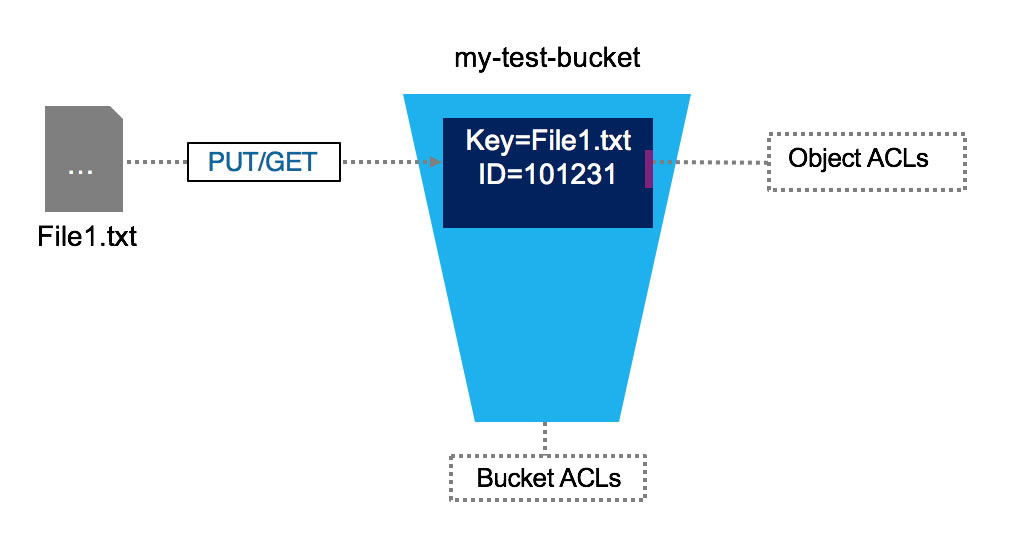
\includegraphics[scale=0.4]{images/object-storage}
	\caption{Komponenten von Objekt Speichern \parencite[S. 5]{Rios.2017}}
	\label{fig:objectstorage}
\end{figure}

Dieser Typ von Dateisystem umfasst drei Hauptkomponente:

\begin{itemize}
	\item \textbf{Daten:}\\
	 Nutzer und Anwendungsinformationen, die persistent hinterlegt werden müssen. Jede Art von Format ist hierbei unterstützt.
	\item \textbf{Metadaten:}\\
	 Diese sind Informationen über die eigentlichen Daten. Beispiele hierfür sind Dateigröße oder Uploadzeit. Ebenfalls können benutzerdefiniert Schlüssel-Wert Paare von nutzenden Anwendungen gespeichert werden. Diese sind von den Applikationen oder Usern zu jeder Zeit frei veränderbar. Eine Besonderheit dieses File Systems ist, dass die Metadaten zusammen mit den eigentlichen Daten gespeichert werden.
	\item \textbf{\ac{UUID}:} Diese eindeutige ID wird jedem Objekt im Speicher zugeordnet. Mit ihr können Daten unterschieden  und gefunden werden, unabhängig von der physikalischen Position der eigentlichen Informationen.
\end{itemize}

Durch obige Eigenschaften wird eine flache Hierarchie erzeugt, die Probleme mit außer Kontrolle geratenen Metadaten Speichern verhindert. Daten können in sogenannten Buckets zusammengefasst werden, um eine logische Strukturierung einzuführen und ebenfalls die Zugriffsrechte von Nutzern einschränken können.  

Da diese Art von Daten fast immer in der Cloud oder auf einem entfernen Server verwendet wird, bieten sich besonders REST Schnittstellen zum Zugriff auf die Daten an \parencite[S. 4f]{Rios.2017}.

\todo{Validate Information for other systems}


\section{Cloud Computing}\label{sec:cloud}

Cloud Computing kann als eine neue Art der Bereitstellung von Programmen, Diensten und Infrastruktur betrachtet werden, die häufig virtualisiert und automatisch skalierbar ist. Es ist die logische Weiterentwicklung von Netzwerk oder Internet Computing und hilft dabei, vorhandene Ressourcen besser auszunutzen. 
Software, Laufzeiten und sogar Plattformen werden in einem verteilten Serverclusters angeboten. Diese können dann von jeder Art  Client Geräten (Personal Computer, Smartphones, \ac{IoT} Devices) angesprochen werden. Außer Anwendungen werden häufig  auch Speicher, bestimmte Dienste oder Entwicklungswerkzeuge über die Cloud angeboten \parencite[S. 3]{furth.2010}.

Ein großer Vorteil von Cloudumgebungen ist die Dezentralisierung von Anwendungen. Statt für eine Applikation einen einzelnen Server zu nutzen, wird diese in einem Netz von diesen virtualisiert. Dieses Netz von Servern kann eine Vielzahl von Anwendungen provisonieren und bei Bedarf automatisch höhere Leistung zuordnen. Hierdurch werden Kosten gespart und eine bessere Verfügbarkeit garantiert \parencite[S. 7]{furth.2010}.

Es gibt einige Schlüsseltechnologien, die Cloud Computing erst ermöglichen. 

Zum einen ist Virtualisierung extrem wichtig, da Container und virtuelle Maschinen auf verschiedenen Servern gehostet werden können (Entkopplung von Anwendung, OS, Hardware und Nutzerdaten), um unterschiedliche Anwendungen für globale Zugriffspunkte bereitzustellen. 
Sobald mehr Performance notwendig ist (mehr Zugriffe), können diese mehr Serverleistung bekommen oder es werden weitere Instanzen auf zusätzlichen Rechnern erzeugt.
Um diese effektiv umzusetzen, besitzen Cloudsysteme einen Load Balancer oder Router, der automatisch Zugriffe auf die bereitstellenden Server verteilt und dafür sorgt, dass zum Beispiel Sitzungen aufrecht erhalten werden (Die Zugriffe eines Nutzer landen immer auf demselben Server).
Zur Loslösung von Speicher wird dieser gerne in separaten \acs{SAN} ausgelagert \parencite[S. 22]{rafaels.2015}.

Wie in \autoref{fig:cloudarchtecture} zu sehen ist, besteht ein Cloud System aus vielen unterschiedlichen Komponenten, verteilt über eine Vielzahl von Servern, um Systemfunktionalitäten über ein \ac{WAN} verfügbar zu machen.   

\begin{figure}[hbt]
	\centering
	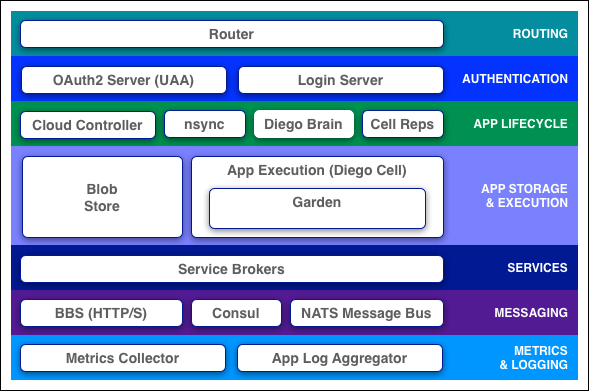
\includegraphics[scale=0.75]{images/cloud-architecture}
	\caption{Hauptkomponenten eines Cloudsystems anhand des Beispiels von Cloud Foundry  \parencite{cloudfoundry.2017}}
	\label{fig:cloudarchtecture}
\end{figure}

%\todo{Check Reference https://w3-connections.ibm.com/blogs/a30b75e7-5fc2-493c-b56b-c94793864a18/entry/ICOS\_Gartner?lang=en\_us}

%Insert General explanation here
\todo{Weitere Quellen benutzen}

Cloud Computing kann als eine neue Art der Bereitstellung von Programmen, Diensten und Infrastruktur betrachtet werden, die häufig virtualisiert und automatisch skalierbar ist. Es ist die logische Weiterentwicklung von Netzwerk oder Internet Computing und hilft dabei vorhandene Ressourcen besser auszunutzen. 
Software, Laufzeiten und sogar Plattformen werden in einem verteilten Serverclusters angeboten. Diese können dann von jeder Art  Client Geräten (Personal Computer, Smartphones, \ac{IoT} Devices) angesprochen werden. Außer Anwendungen werden häufig  auch Speicher, bestimmte Dienste oder Entwicklungswerkzeuge über die Cloud angeboten \parencite[S. 3]{furth.2010}.

Ein großer Vorteil von Cloud Umgebung ist die Dezentralisierung von Anwendungen. Statt für eine Applikation einen einzelnen Server zu nutzen, wird diese in einem Netz von diesen virtualisiert. Dieses Netz von Servern kann eine Vielzahl von Anwendungen provisonieren und bei Bedarf automatisch höhere Leistung zuordnen. Hierdurch werden Kosten gespart und eine bessere Verfügbarkeit garantiert \parencite[S. 7]{furth.2010}.

Es gibt einige Schlüsseltechnologien die Cloud Computing erst ermöglichen. 

Zum einen ist Virtualisierung extrem wichtig, da Container und virtuelle Maschinen auf verschiedenen Servern gehostet werden können (Entkopplung von Anwendung, OS, Hardware und Nutzerdaten), um unterschiedliche Anwendungen für globale Zugriffspunkte bereitzustellen. 
Sobald mehr Performance notwendig ist (mehr Zugriffe) können diesen mehr Serverleistung bekommen oder es werden weitere Instanzen auf zusätzlichen Rechnern erzeugt.
Um diese effektiv umzusetzen besitzen Cloud Systeme einen Load Balancer, der automatisch Zugriffe auf die bereitstellenden Server verteilt und dafür sorgt, dass zum Beispiel Sitzungen aufrecht erhalten werden (Die Zugriffe eines Nutzer landen immer auf dem selben Server).
Zur Loslösung von Speicher wird dieser gerne in separaten \acs{SAN} ausgelagert \parencite[S. 22]{rafaels.2015}.
\subsection{Cloud Modelle}
%On/Off Premise
%SaaS / PaaS / IaaS

Es gibt verschiedene Cloud Modelle, die jeweils unterschiedliche Features für den User bereitstellen. Hauptsächlich unterscheidet man hier zwischen \ac{IaaS}, \ac{PaaS} und \ac{SaaS}, welche aber auch gleichzeitig vom selben Anbieter zur Verfügung stehen können.

\begin{itemize}
	\item \textbf{IaaS}:\\
	Dem Nutzer hat die Kontrolle über das zu verwendende OS, den Speicher und gehostete Anwendungen. Nur die unterliegende Cloud Infrastruktur ist nicht veränderbar und häufig sind auch nur bestimmte Teile der Firewall anpassbar.
	\item \textbf{PaaS}:\\
	In diesem Fall hat der Nutzer keine Wahl was Betriebssystem, Netzwerk Fähigkeiten oder Speicher angeht, es existiert eine vorinstallierte Umgebung (Datenbanken, Frameworks, Laufzeiten, usw.) zum Ausführen von eigenen Applikationen. Begrenzt bestehen Konfigurationsmöglichkeiten für die Hosting Umgebung der Software. 
	\item \textbf{SaaS}:\\
	Es wird nur eine bestimmte Anwendung oder Interface dem Nutzer offengelegt. Er kann diese verwenden und ggf. seine persönliche Instanz konfigurieren, hat aber keinerlei Kontrolle über die unterliegend Laufzeit Umgebungen, den Speicher, das Netzwerk oder das OS \parencite[S. 15f]{rafaels.2015}.
\end{itemize}

Des weiteren können Cloud Server in verschiedenen Umgebungen installiert werden, um Zugriff, Sicherheit und Verfügbarkeit zu regulieren.

\begin{itemize}
	\item \textbf{Public Cloud}:\\
	Die Cloud Server sind öffentlich zugänglich und jeder kann Anwendungen erstellen und über die Infrastruktur bereitstellen. Das System wird meistens von einer Firma oder Regierungsstelle betrieben und die notwendige Hardware steht auf dessen Gelände. 
	\item \textbf{Private Cloud}:\\
	Die gesamte Cloud Infrastruktur wird nur für einen Kunden zur Verfügung gestellt und ist nur für diesen zugänglich. Sie kann von ihm oder einer dritten Gruppen gemanagt werden. Es besteht die Möglichkeit das System auf dem Gelände des Käufers zu installieren, um zum Beispiel Datensicherheit von kritischen Informationen zu gewährleisten. 
	\item \textbf{Hybrid Cloud}:\\
	Eine Hybrid Cloud verbindet Elemente aus einem öffentlichen und privaten Setup. Zum Beispiel können Teile der Berechnung in der public Cloud stattfinden und Personaldaten auf den privaten Servern verbleiben. Hierdurch können Datenschutz Bedenken berücksichtigt und die Vorteile öffentlichen Cloud Computings ausgenutzt werden. Zur Kommunikation zwischen den beiden Server Clustern können verschiedene standardisierte Schnittstellen verwendet werden (z.B. REST)  \parencite{rafaels.2015}.
\end{itemize}

\subsection{Anbieter}
Durch die Popularität von Cloud Computing gibt es mittlerweile an Vielzahl von Anbietern, an dieser Stelle werden nur die drei Größten (1. Amazon Web Services, 2. Microsoft, 3. IBM) kurz vorgestellt \parencite{statistia.2016}. Es wird sich hierbei auf Anbieter beschränkt, die mindestens \acs{PaaS} Funktionalitäten bieten, da für das Projekt dieser Arbeit eigene Anwendungen entwickelt werden müssen.


\textbf{Amazon Web Services}\\
Amazon ist im Moment der Marktführer mit fast 30 Prozent Marktanteil. Dies basiert zum einen darauf, dass \ac{AWS} er mit einer der ersten modernen Anbieter (seit 2002 in einfacher Form und seit 2006 mit den ersten Cloud Services) ist und es eine Vielzahl von Diensten gibt. Es gibt sowohl direkt ansprechbare Services für Speicher, Rechenleistung und Netzwerk Fähigkeiten für \acs{PaaS} Aufgaben als auch VM Systeme und Container für frei konfigurierbare Anwendungen (\acs{IaaS}).

Zum Beispiel die \ac{S3} Schnittstelle wurde von Amazon entwickelt und wird an einer Vielzahl von Stellen für die Kommunikation mit Objekt Speichersystemen verwendet \parencite{aws.2017}.

Aufgrund Amazons langer Geschichte mit Cloud Computing bieten sie im Moment die meisten Datencenter weltweit an und haben mehr Rechenleistung als die beiden anderen Konkurrenten zusammen. Auch bei der Auswahl von Diensten, haben Entwickler hier die meiste Vielfalt. Als Nachteil gelten eine gewisse Komplexität bei der Nutzung und eine Vernachlässigung des Hybrid und Privat Cloud Angebots \parencite{computerworlduk.2016}.


\textbf{Microsoft Azure}\\
Azure ist die Anwendungsplattform von Microsoft für eine öffentliche Cloud mit \acs{PaaS} und \acs{IaaS} Features. Sie ist spezialisiert für die Kombination mit Microsoft Diensten, Programmiersprachen und Lösungen. Mithilfe eines Management Portals lassen sich gehostete Applikationen verwalten. 

Es besteht die Möglichkeit \ac{VM}s oder Web Applikationen, für die eine Bandbreite an verschiedenen Diensten zur Verfügung steht, zu erzeugen. Es können ganze \acs{VM}s, Container oder auch nur einzelne lokale Komponenten (z.B. Speicher )aus on-premise Datencentern leicht in die Cloud gehoben werden.

Insgesamt gibt es viele Überschneidungen mit \acs{AWS}, aber die Kompatibilität mit Microsoft/Windows Komponenten ist wesentlich höher und andere Lösungen sind weniger vertreten \parencite{microsoft.2015}.


\textbf{IBM Bluemix}\\
Bei Bluemix handelt es sich um die \acs{PaaS}/\acs{IaaS} (wobei diese Funktion von Softlayer zur Verfügung gestellt werden) Lösung von IBM, die zuerst 2014 das erste Mal vorgestellt wurde. Außer der Möglichkeit \acs{VM}s, Root Server und Docker Container zu hosten, werden eine Vielzahl von IBM und Drittpartei Dienste angeboten, die von Speicher bis zu \acs{IoT} oder Maschinen Lernen reichen.

Es kann in einer Vielzahl populärer Sprache entwickelt werden (Node, PHP, Ruby, Java, Go...) und es gibt so genannte Buildpacks, die nicht vorhandene Laufzeit Umgebungen zum Teil nachrüsten. Ebenfalls kann Bluemix als private Cloud oder in einem "dedizierten" Modus zur Verfügung gestellt werden. Bei diesem wird garantiert, dass eine \acs{VM} nur auf einem isolierten Bare-Metal Server läuft.

In der Bluemix Konsole (Management Oberfläche) lassen sich auch einige \gls{DevOps} Funktionen konfigurieren. Es gibt einen eigenen Code Editor, Gitlab Integration und eine Buildpipeline für \ac{CI} \parencite{fassnacht.2016}.

Im Vergleich zur Konkurrenz bietet IBM viele \acs{IaaS} Dienste, kann aber bei Funktionen für Entwickler von Anwendungen nicht mithalten \parencite{computerwoche.2016}. 

\subsection{Entwicklung in einem Cloud System} \todo{Maybe remove or move to chapter 3}
		
	% Planung
	\chapter{Methoden}\label{ch:methods}

In diesem Kapitel werden notwendige Komponenten der zu entwickelnden Hybrid Cloudlösungen ausgewählt und begründet. Ebenfalls werden Techniken beschrieben, die bei der Entwicklung der Demoapplikation verwendet werden. 

Einschränkungen bei der Wahl von Lösungen sind aufgrund der Umgebung \ref{subsec:enviroment} vorhanden und werden entsprechend hier gekennzeichnet und diskutiert.

\section{Auswahl des verteilten Dateisystems}
Bei der Wahl des Dateisystems müssen die ursprünglichen Anwendungsszenarien von Hadoop und Spectrum Scale betrachtet werden. 

Apache Hadoop soll dafür verwendet werden, Operationen auf möglichst effiziente Weise in einem verteilten System ausführen. \acs{HDFS} stellt hierbei die Speicherkomponente dar und baut auf normalen ext4 Dateisystemen auf. Dies macht insbesondere Sinn, da Hadoop Cluster meistens aus gewöhnlicher Hardware bestehen. Nachteil hiervon ist ein erschwerter Zugriff, da auf das System mit einem speziellen Befehlsset immer von außen zugegriffen und eine Datenveränderung erst innerhalb der geschachtelten Systeme ausgetauscht werden muss.
Hadoop ist Open Source und kann somit kostenlos verwendet werden \parencite{snowflake.2016}. 

Spectrum Scale hingegen war ursprünglich als proprietärer High-Performance Speichersystem für jede Art von Anwendung entworfen worden. Es kann alle mögliche Arten von Storagetypen (\acs{SAN}, \acs{NAS}, \acs{DAS}) anbinden und diese über eine einheitliche Schnittstelle dem Nutzer zur Verfügung stellen. Die verschiedene Hardware kann abgestuft werden, sodass alte oder kalte Daten auf langsame Speicher verschoben oder in die Cloud gespeichert werden.  Durch die \gls{POSIX} Konformität von \acs{GPFS} ist ein einfaches Navigieren sämtlicher Dateien im Cluster möglich und Veränderungen werden direkt angewendet \parencite{snowflake.2016}.

Insgesamt gewinnt \acs{GPFS} im Sinne von Performance, da es ein Kernel-Level-Dateisystem ist, auf das wesentlich schneller zugegriffen werden kann. Es existieren Erweiterungen für Cloud Tiering und Sharing, die in dieser Form nicht bei HDFS existieren. Jede Art von Anwendung kann durch \acs{GPFS} profitieren, auch klassische Anwendungen, die nicht in einem verteilten System laufen.

Außerdem entfallen mögliche Kosten von Spectrum Scale, da diese Arbeit in einer IBM-Abteilung angefertigt wird und somit einfacher Zugriff auf die Software besteht.

Aus den oben diskutierten Gründen wird in dieser Arbeit \textbf{IBM Spectrum Scale} verwendet.

\section{Auswahl des Cloud Anbieters}

Bei der Auswahl des Cloudanbieters sind einige Punkte zu beachten. Zum einen sollten \acs{PaaS} Funktionalitäten gegeben sein, damit eine vollständige Anwendung entwickelt und hochgeladen werden kann und zum anderen sollte ein Service vorhanden sein, der als Cloudspeicher mit dem zuvor ausgewählten Spectrum Scale kombinierbar ist.
Cloud Tiering und Sharing sind einsetzbar mit allen S3-konformen Objekten Speichern \parencite[S. 110]{ibm.2017}. 

Diese beiden Punkte sind bei allen drei Anbietern erfüllt.

Bei \acs{GPFS} kann zusätzlich noch ein IBM eigenes Format verwendet werden, um die Daten zwischen dem lokalen und Cloud System auszutauschen.
Von der Netzwerkgröße und Verfügbarkeit gewinnt \acs{AWS}, da es die meisten Server weltweit und auch speziell in Deutschland bereitstellt. Trotzdem sind ebenfalls Server von Microsoft und IBM in Deutschland vorhanden, sodass keine wesentlichen Nachteile entstehen.

Microsoft Azure lässt sich in optimaler Form (ohne das Aufsetzen einer dedizierten \acs{VM}) mit .NET-Laufzeiten benutzen, was die Auswahl der Entwicklungswerkzeuge wesentlich einschränkt.

Bluemix bietet einige DevOps-Features an, die die Entwicklung massiv beschleunigen, das Aufsetzen einer Anwendung auf \acs{AWS} kann sich als komplizierter erweisen.

Zusätzlich entfallen sämtliche Kosten bei IBM Bluemix, da ein firmeninterner Account genutzt werden kann und auch zusätzliche Kosten für weitere verwendete Dienste entfallen.

Besonders aus letzterem Grund, obwohl AWS oder Azure nicht ungeeigneter sind, wird für die Entwicklung der Demo \textbf{IBM Bluemix} verwendet.

\section{Demoentwicklung - Auswahl der Laufzeitumgebung und Dienste}

Wie in \autoref{subsec:cloudprovider} beschrieben wurde, stellen \acs{PaaS}-Umgebungen verschiedene Laufzeitumgebungen zur Verfügung. Zusätzlich wird eine Vielzahl von Diensten angeboten, um klassische Probleme wie Speicher, Kommunikation oder Analytics zu lösen.

An dieser Stelle wird kurz beschrieben, welche Produkte zur Erstellung der Demoapplikation verwendet werden. 

Als Entwicklersprache wird node.js Version 7.5.0 verwendet. Node ist eine auf der Chrome V8 basierende Javascript Engine. Sie verwendet ein nicht blockierendes I/O-Modell, dass besonders gut für parallel auftretende Netzwerkanfragen eingesetzt werden kann. In Kombination mit dieser Sprache wird der \ac{npm} benutzt \parencite{nodejs.2017}.

Zur Erweiterung der Serverfähigkeiten von Node.js wird express verwendet. Dies ist ein Framework zur Entwicklung von Webanwendungen, dass eine Vielzahl nützlicher Middleware unterstützt.

Zur Versionsverwaltung wird \gls{Git} verwendet, auf welches auch die \ac{CD} Pipeline von Bluemix zugreift. Diese lädt den Quellcode aus dem Repository herunter, installiert die notwendigen Abhängigkeiten (Diese werden bei \acs{npm} in einer Paketbeschreibungsdatei hinterlegt: \textit{package.json}) und verschiebt die fertig gebaute Anwendung in das Cloud Foundry Servernetzwerk.  

Alle späteren Änderungen auf dem \textit{develop} Entwicklungszweig werden automatisch in Bluemix über dem oben beschrieben Weg angewendet. Über die grafische Oberfläche von Bluemix können zusätzliche Dienste konfiguriert werden.

Zur Kommunikation mit der S3 Schnittstelle des \acs{COS} wird ein Abstraktion der \acs{AWS} \gls{SDK} verwendet. Mithilfe von dieser kann mit allen \acs{S3} kompatiblen Diensten kommuniziert werden.

Desweiteren werden folgende, im Projekt wichtige, offene Bibliotheken verwendet:

\begin{table}
	\centering
		\begin{tabular}{ l | c | p{8cm}}
			\hline
			Paketname & Version & Beschreibung \\ \hline
			Node.js & 7.5.0 & Javascript Laufzeitumgebung \\
			Express & 4.15 & Framework für Webanwendungen \\
			JQuery & 3.2.1 & Eine Sammlung von Werkzeugen, um auf unterschiedlichen Browsern javascript-Aufgaben zu vereinheitlichen \\
			Bootstrap & 3.3.7 & Grafik Framework, um responsive Webseiten zu designen. \\
			Moment & 2.18.1 & Bibliothek zum Umgang mit Zeitzonen und generellen Zeitberechnungen \\
			Filesize & 3.5.10 & Bibliothek zur automatischen Konvertierung von Dateigrößen \\
			aws-sdk & 2.87.0 & AWS SDK, wird verwendet um S3 kompatible Dienste anzusprechen \\
			ejs & 2.5.6 & HTML-ähnliches Template zur Verwendung mit Express \\
			body-parser & 1.17.2 & Express Middleware zum Parsen von HTTP Körpern in unterschiedlichen Formaten (z.B. JSON)\\
			Morgan & 1.8.2 & Logging Middleware für HTTP-Anfragen in express \\
			Multer & 1.3.0 & Middleware zum Umgang mit Multipart/Datei Uploads von Clientanwendungen \\
			Toastr & 2.1.2 & Frontend Bibliothek zum Erzeugen von Toast-Nachrichten \\
			Watson Developer Cloud & 2.34.0 & Modul zum Zugriff auf verschiedenen Watson Dienste, in diesem Fall wird Ein Bildanalyse Tool eingebunden \\
			mkdirp & 0.5.1 & Backend Bibliothek zum Erzeugen von Ordnerhierarchien
		\end{tabular}
		\caption{Verwendete NPM-Pakete}
		\label{tab:npmpackages}
\end{table}

	
	% Setup
	\chapter{Umsetzung und Implementierung}\label{ch:realization}
	
	% Schlussbetrachtung
	\chapter{Schlussbetrachtungen}\label{ch:conclusion}

In diesem Kapitel werden die praktischen Ergebnisse der Arbeit kritisch beleuchtet und diskutiert, um Vorteile und Nachteile eines solchen Projektes herauszustellen. Außerdem wird ein kurzer Ausblick auf zukünftige Entwicklungen in diesem Feld gegeben.

\section{Diskussion der Ergebnisse}
Anhand der Implementierung einer einfachen Hybrid-Cloud Lösung lassen sich bereits einige allgemeingültige Schlüsse ableiten:

Es ist möglich, Clusterspeicher mithilfe von Cloud Computing zu kombinieren, ohne dass hierfür eine Vielzahl an neuen Technologien entwickelt werden muss. Bestehende Software lässt sich kombinieren und hiermit eine Brücke zwischen Anwendungen in einer privaten und öffentlichen Cloud erzeugen. Es gibt verschiedene Möglichkeiten (zum Beispiel Cloud-Tiering oder Data Sharing), Daten mit der Cloud auszutauschen, ohne dass hierfür das aktuelle lokale Speichersetup verändert werden muss.
Dieses kann also auch weiterhin schnelle Platten oder \acp{SSD} für I/O intensive Aufgaben verwenden und nur kalte Daten in die Cloud senden.
Einmal exportierte Daten sind leicht zugänglich, da aufgrund des \ac{S3} Protokolls ein einheitlicher Standard zum Zugriff auf die Daten gegeben ist. Für diesen gibt es auch eine Vielzahl von Clientenprogrammenund Entwicklungspakete (SDK) für alle relevanten Programmiersprachen.
Sie können somit von einer Vielzahl von anderen Anwendungen sehr leicht verwendet werden. Diese können dann auch auf Dienste zugreifen, die nur über bestimmte öffentliche Cloudplattformen verfügbar sind (Der verwendete Watson Dienst ist ein Beispiel hierfür).

Trotz allem ist das gesamte Setup sehr aufwendig, da sowohl Komponente auf den privaten Servern wie auch in der Cloud Umgebung erzeugt werden müssen. Es besteht also ein doppelter Administrationsaufwand, der nur schwer vermieden werden kann. 
Zusätzlich bestehen auf der Seite von IBM Spectrum Scale keine dedizierten Funktionen zum direkten Erstellen eines Manifests aus einem Cloudobjektspeicher.. Daten, die in der Cloud erzeugt werden, können nur über Umwege wieder zurück in den Speichercluster importiert werden. Dies macht es notwendig, dass hierfür eigene Software entwickelt wird.
Durch die Verwendung von \ac{COS} entsteht ebenfalls ein Leistungsflaschenhals, da Dateien nur mithilfe des HTTP-Protokolls hoch- oder heruntergeladen werden können. Bei diesem entstehen für jede Anfrage unnötig große Überhänge, da mehrere Schichten an Kopfdateien angehängt werden. Aufseiten von Scale können natürlich mehrere Import- oder Exportvorgänge parallel stattfinden, dies ist aber nicht unbedingt für die konsumierende Cloudanwendung gegeben. Bei dieser müsste eine Parallelität manuell implementiert werden, was je nach verwendeter Sprache sehr aufwendig ausfallen kann.
Mit dieser Art von Hybrid-Cloud kann niemals eine Echtzeitaustausch von Daten stattfinden. Sie müssen erst von Scale in \ac{COS} exportiert und dann von der öffentlichen Anwendung heruntergeladen werden. In die andere Richtung muss Scale erst über die Veränderung benachrichtigt werden, damit dieses dann die veränderte Datei herunterladen kann. Trotzdem stellt diese im Moment den aktuellen Stand der Technik dar und ist normal für Hybrid-Cloud Anwendungen.

Trotz der oben genannten Einschränkungen ist der Aufbau wertvoll. Ein Beispiel hierfür wären typische \ac{BI} oder Data-Mining Anwendungen. Die Daten des Geschäftstages können nachts hochgeladen und dann analysiert werden.
Geschützte Daten könnten bereinigt und nur allgemeine Angaben in die Cloud für Analysezwecke hochgeladen werden.
Ebenfalls macht dieses Setup auch die Sicherung von Daten möglich, da Cloudspeicher im Normalfall sehr günstig ist.

Es ist also möglich eine Vielzahl von neuen Anwendungsgebieten zu erschließen, die so mit einer rein privaten oder öffentlichen Cloud nicht möglich ist. Trotz Einschränkungen lässt sich mit gewissem Aufwand eine zuverlässige, stabile und schnell laufende Anwendung erzeugen. 
\section{Fazit \& Ausblick}

An dieser Stelle wird kurz untersucht inwiefern, die am Anfang gestellten Anforderungen erfüllt und umgesetzt wurden.

\subsection{Reflexion der Aufgabenstellung und Zielerreichung}

Ziel der Arbeit ist die Anbindung von IBMSpectrum Scale an eine öffentliche Cloudplattform, speziell IBM Bluemix. Um dies zu erreichen, müssen verschiedene Technologien für Speicher und Cloud-Computing untersucht und die in diesem Kontext beste ausgewählt werden. Nach dieser theoretischen Untersuchung sollen ein Testcluster, ein Cloudspeicher und alle notwendigen Komponenten für die Demo erstellt werden.
Die Applikation soll zusätzlich einen Clouddienst einbinden, der eine nicht triviale Funktionalität umsetzt. Ansonsten soll diese ein einfaches Nutzerinterface für Vorführungszwecke besitzen.

\textbf{Zielerreichung:}\\
Oben genannte Ziele wurden voll erreicht. Nach Untersuchung von verschiedenen Techniken für Cloud und Speicher hat sich IBM Bluemix in Kombination mit \ac{COS} als beste für die Demo erwiesen. 

Es wurde ein angepasstes VM-Abbild erzeugt, mithilfe dem ein IBM Spectrum Scale Cluster aufgesetzt werden kann, der fertig für Cloud Sharing mithilfe von \acl{COS} konfiguriert ist. Ebenfalls wurde eine Anwendung (basierend auf einer node.js Laufzeitumgebung) auf Bluemix erstellt, die Einsicht und Analyse von Bilddateien auf \ac{COS} ermöglicht. Diese verwendet hierfür einen Watson Service aus dem Bluemix-Service-Katalog. Die Analysedaten werden den ursprünglichen Dateien als Metainformationen hinzugefügt und stehen dann auch wieder IBM Spectrum Scale zur Verfügung 

Das Aufsetzen der Lösung im Labor ist nicht notwendig, da die Rechenleistung eines normalen Bürodesktops ausreicht, um die Demo darzustellen. Zudem kann die Demo auch vorgeführt werden, wenn die eigentliche IBM Spectrum Scale Instanz heruntergefahren oder nicht erreichbar ist.

\subsection{Ausblick für zukünftige Entwicklungen}
In dem aktuellen Aufbau werden keine wirklichen Anwendungen in der privaten Komponente ausgeführt, was aber ohne weiteres möglich wäre. Es könnten zum Beispiel auf einzelnen Knoten des GPFS-Clusters eigene Anwendungen laufen, die Daten konsumieren und produzieren. Diese könnten dann immer zu einem festen Zeitpunkt in \ac{COS} synchronisiert und dort weiter analysiert werden.
Analysierte Bilder werden aktuell mit Metadaten von der Cloudanwendung bereichert, die aber ansonsten noch keine Verwendung finden. Diese könnten ebenfalls wieder auf der IBM Spectrum Scale Seite Weiterverwendung finden. 

Ebenfalls lässt sich die Cloudanwendung noch beliebig erweitern. Es könnten weitere Analysedienste verwendet oder eine komplett andere Anwendung eingesetzt werden.

Die einzelnen Komponente dieser Arbeit (IBM Spectrum Scale Abbild, Demo-Express-Server, Demofrontend) sind so gestaltet, dass sie auch einzeln weiterverwendet werden können. Das Clusterspeichersystem kann zum Beispiel auch mithilfe anderer Objektspeicher verwendet werden oder es kann statt Cloud Data Sharing Cloud Tiering zum Auslagern der Daten verwendet werden.

Alles in allem erfüllt die Demo ihre Aufgabe, Möglichkeiten eines Hybrid-Cloud Setups zu zeigen und somit Entwicklungen für andere Projekte zu inspirieren. 

	\clearpage
	\listoftodos
		
	\pagenumbering{roman}
	
	% Literaturverzeichnis
	\cleardoublepage
	\printbibheading
	\printbibliography[nottype=online,heading=subbibliography,title={Publikationen}]
	\printbibliography[type=online,notkeyword=Gesetz,notkeyword=Standard,heading=subbibliography,title={Online Quellen}]
%	\printbibliography[type=online,keyword=Gesetz,heading=subbibliography,title={Rechtsquellenverzeichnis}]
%	\printbibliography[type=online,keyword=Standard,heading=subbibliography,title={Standards \& Normen}]
	
%	\renewcommand\bibname{Literaturverzeichnis}
%	\printbibliography

%	\newpage\null\thispagestyle{plain}\newpage
	
	% Glossar
	\printglossary[style=altlist,title=\langglossar]
	
	% sonstiger Anhang
	\clearpage
	\appendix
	%% !TeX root = ../dokumentation.tex

\addchap{\langanhang}

{\Large
\begin{enumerate}[label=\Alph*.]
	\item Screenshot NameNode Web-Interface
	\item DVD Inhalt
	\item DVD 
\end{enumerate}
}
\pagebreak

\section*{A. Screenshot NameNode Web-Interface}\label{sec:ScreenNameNodeWeb}
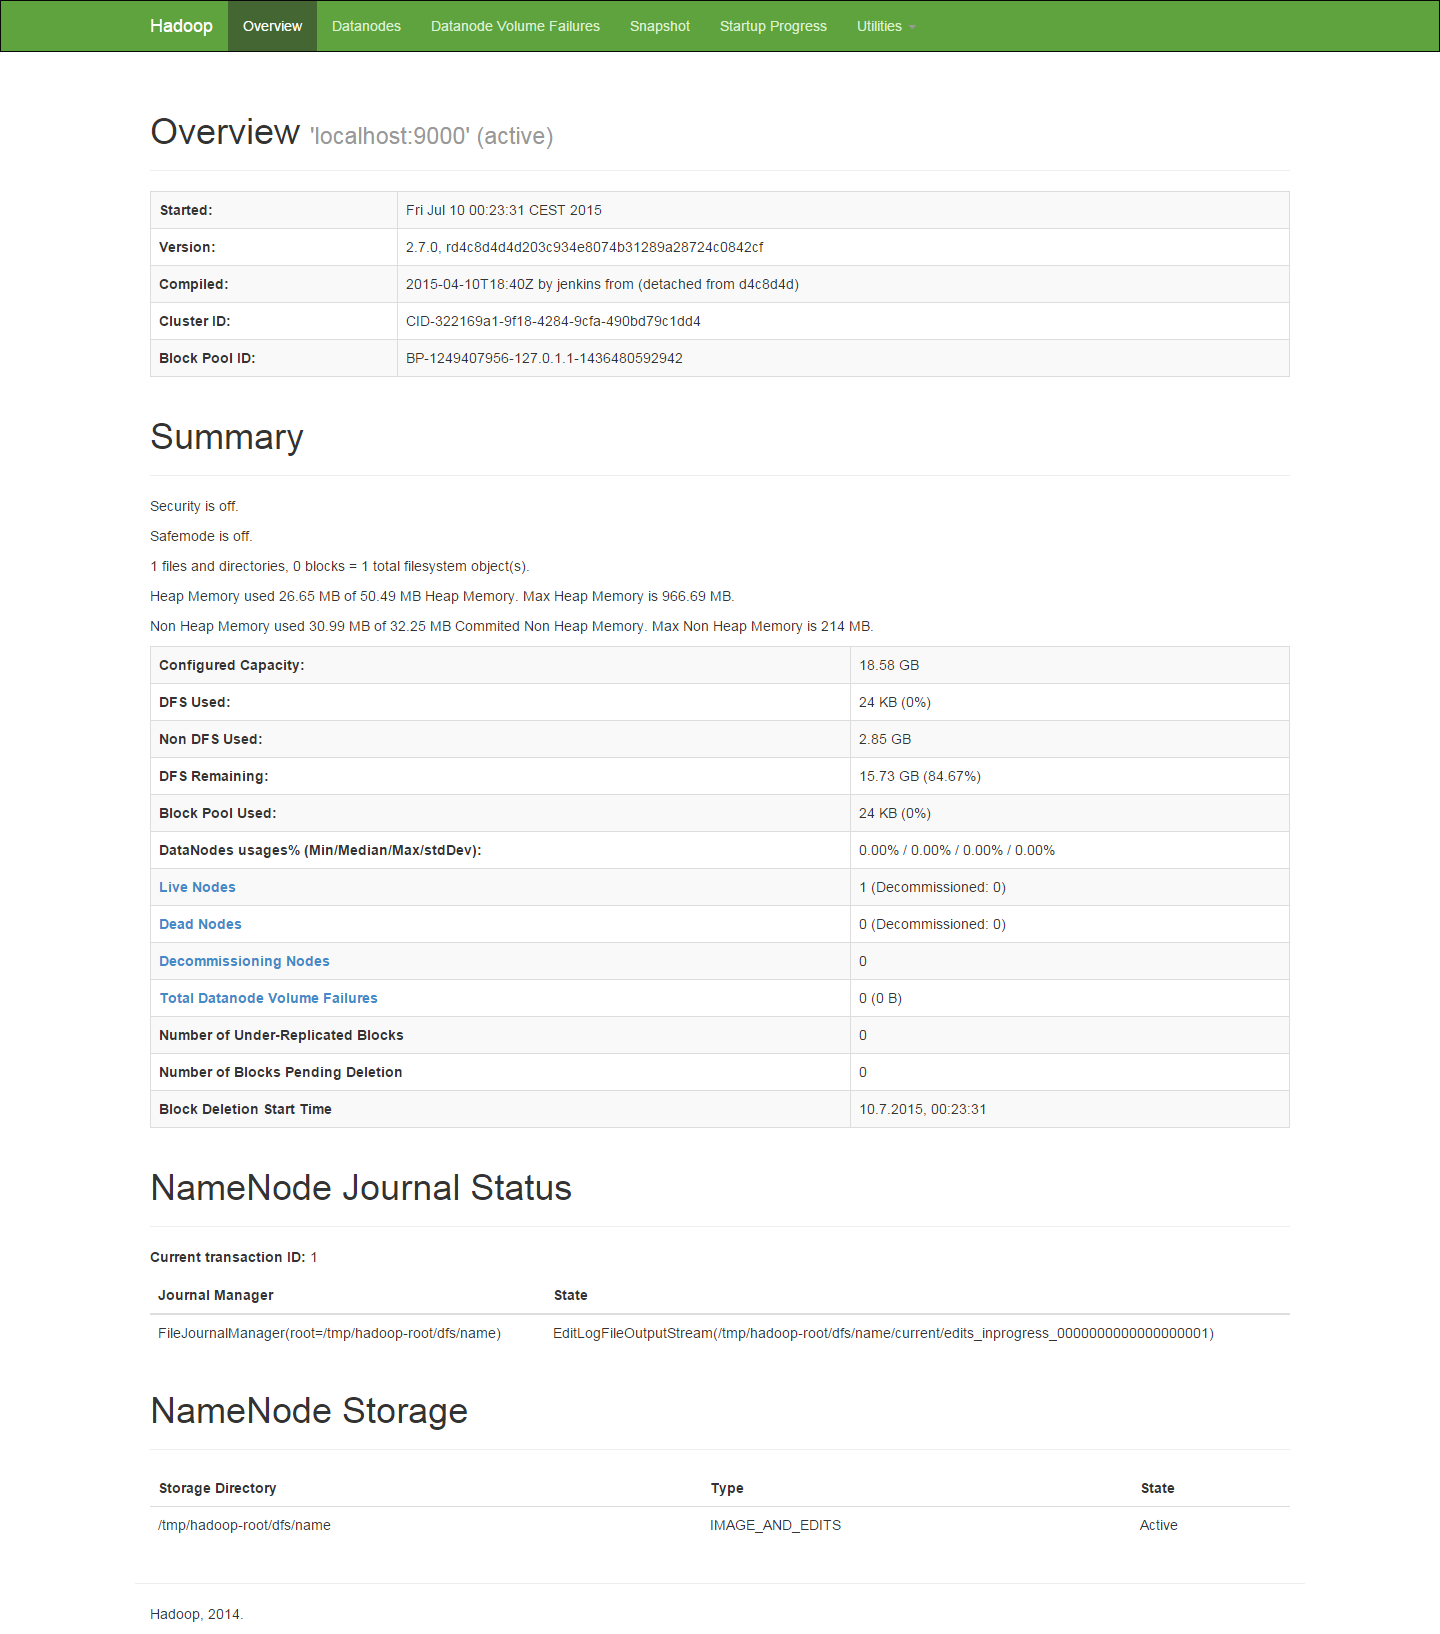
\includegraphics[width=1\textwidth]{NameNodeWebInterface.png}
\pagebreak

\section*{C. DVD Inhalt}
\begin{tabbing}
	mm \= mm \= mm \= mmmmmmmmmmmmmmmmmm \= \kill
	$\vdash$ \textbf{Anwendung/} \\ 
	| \> -- pom-xml \> \> \> $\Rightarrow$ \textit{Maven POM Datei} \\
	| \> $\vdash$ \textbf{conf/} \> \> \> $\Rightarrow$ \textit{*.properties Dateien für Konfiguration} \\
	| \> $\vdash$ \textbf{src/} \> \> \> $\Rightarrow$ \textit{Quellcode Dateien} \\
	| \> $\vdash$ \textbf{target/} \\
	| \> | \> -- Logfileanalyzer-1.0-SNAPSHOT.jar \> \> $\Rightarrow$ \textit{Ausführtbare JAR-Datei} \\
	| \> | \> $\vdash$ \textbf{site/apidocs/} \> \> $\Rightarrow$ \textit{JavaDoc für Browser} \\
	| \\
	$\vdash$ \textbf{Literatur/} \> \> \> \> $\Rightarrow$ \textit{PDF Literatur \& E-Books} \\
	$\vdash$ \textbf{Praesentationen/} \\
	| \> -- Abschlusspraesentation.pptx \> \> \> $\Rightarrow$ \textit{Präsentation vom 21. August 2015} \\
	| \> -- Abschlusspraesentation.pdf \\
	| \> -- Kickoffpraesentation.pptx \> \> \> $\Rightarrow$ \textit{Präsentation vom 03. Juni 2015} \\
	| \> -- Kickoffpraesentation.pdf \\
	| \\
	$\vdash$ \textbf{Sonstiges/} \\
	| \> -- LineareRegression.xlsx \> \> \> $\Rightarrow$ \textit{Berechnung der linearen Regression} \\
	| \\
	$\vdash$ \textbf{Latex-Files/} \> \> \> \> $\Rightarrow$ \textit{Editierbare \LaTeX~Dateien der Arbeit}\\ %\llcorner
	\> -- bibliographie.bib \> \> \> $\Rightarrow$ \textit{Literaturverzeichnis} \\
	\> -- dokumentation.pdf \> \> \> $\Rightarrow$ \textit{Bachelorarbeit als PDF} \\
	\> -- dokumentation.tex \> \> \> $\Rightarrow$ \textit{Hauptdokument} \\
	\> -- einstellungen.tex \> \> \> $\Rightarrow$ \textit{Einstellungen} \\
	\> $\vdash$  \textbf{ads/}   	\> \> \> $\Rightarrow$ \textit{Header, Glosar, Abkürzungen, etc.}\\
	\> $\vdash$  \textbf{content/}  \> \> \> $\Rightarrow$ \textit{Kapitel}\\
	\> $\vdash$  \textbf{images/}   \> \> \> $\Rightarrow$ \textit{Bilder}\\
	\> $\vdash$  \textbf{lang/}  \> \> \> $\Rightarrow$ \textit{Sprachdateien für \LaTeX~Template}\\
	\> 
\end{tabbing}

	
\end{document}
